\documentclass[aspectratio=169,11pt]{beamer}

\usetheme{Madrid}
\usecolortheme{default}
\usefonttheme{professionalfonts}
\usepackage[T1]{fontenc}
\usepackage{lmodern}
\usepackage{microtype}
\usepackage{graphicx}
\usepackage{booktabs}
\usepackage{siunitx}
\usepackage{amsmath}
\usepackage{xcolor}
\usepackage{hyperref}

\definecolor{airwayblue}{RGB}{25,76,120}
\definecolor{airwayteal}{RGB}{25,125,120}
\setbeamercolor{structure}{fg=airwayblue}
\setbeamercolor{frametitle}{fg=white,bg=airwayblue}
\setbeamercolor{title}{fg=white,bg=airwayblue}
\setbeamercolor{block title}{fg=white,bg=airwayteal}
\setbeamercolor{block body}{bg=airwayteal!8}
\setbeamertemplate{navigation symbols}{}
\setbeamertemplate{caption}[numbered]
\setbeamertemplate{footline}{%
  \leavevmode\hbox{%
    \begin{beamercolorbox}[wd=.78\paperwidth,ht=2.5ex,dp=1ex,leftskip=1em]{author in head/foot}%
      Henri Van Overmeire \hspace{1em} Patient-specific airway CFD
    \end{beamercolorbox}%
    \begin{beamercolorbox}[wd=.22\paperwidth,ht=2.5ex,dp=1ex,center]{date in head/foot}%
      \insertframenumber/\inserttotalframenumber
    \end{beamercolorbox}}}

\graphicspath{{../report/figures/}}
\sisetup{detect-all,per-mode=symbol}

\title{Patient-Specific Computational Fluid Dynamics of the Airways}
\subtitle{Segmentation, mesh generation, and flow analysis in tracheomalacia}
\author{Henri Van Overmeire}
\institute{Computational Biofluid Mechanics}
\date{\today}

\begin{document}

\begin{frame}
  \titlepage
  \vspace{-1em}
  \centering
  \href{https://github.com/henrivanovermeire/tracheomalacia_cfd}{\texttt{github.com/henrivanovermeire/tracheomalacia\_cfd}}
\end{frame}

\begin{frame}{Clinical and computational question}
  \begin{columns}[T,onlytextwidth]
    \column{0.55\textwidth}
      \begin{itemize}
        \item Tracheomalacia and congenital stenosis can strongly increase airway resistance.
        \item CT describes anatomy; CFD estimates velocity, pressure loss, resistance, and flow division.
        \item Preoperative and postoperative anatomy were reconstructed at corresponding tracheal locations.
      \end{itemize}
      \begin{block}{Main question}
        How does the intervention alter lumen calibre and the geometry-driven airflow through the reconstructed airway?
      \end{block}
    \column{0.42\textwidth}
      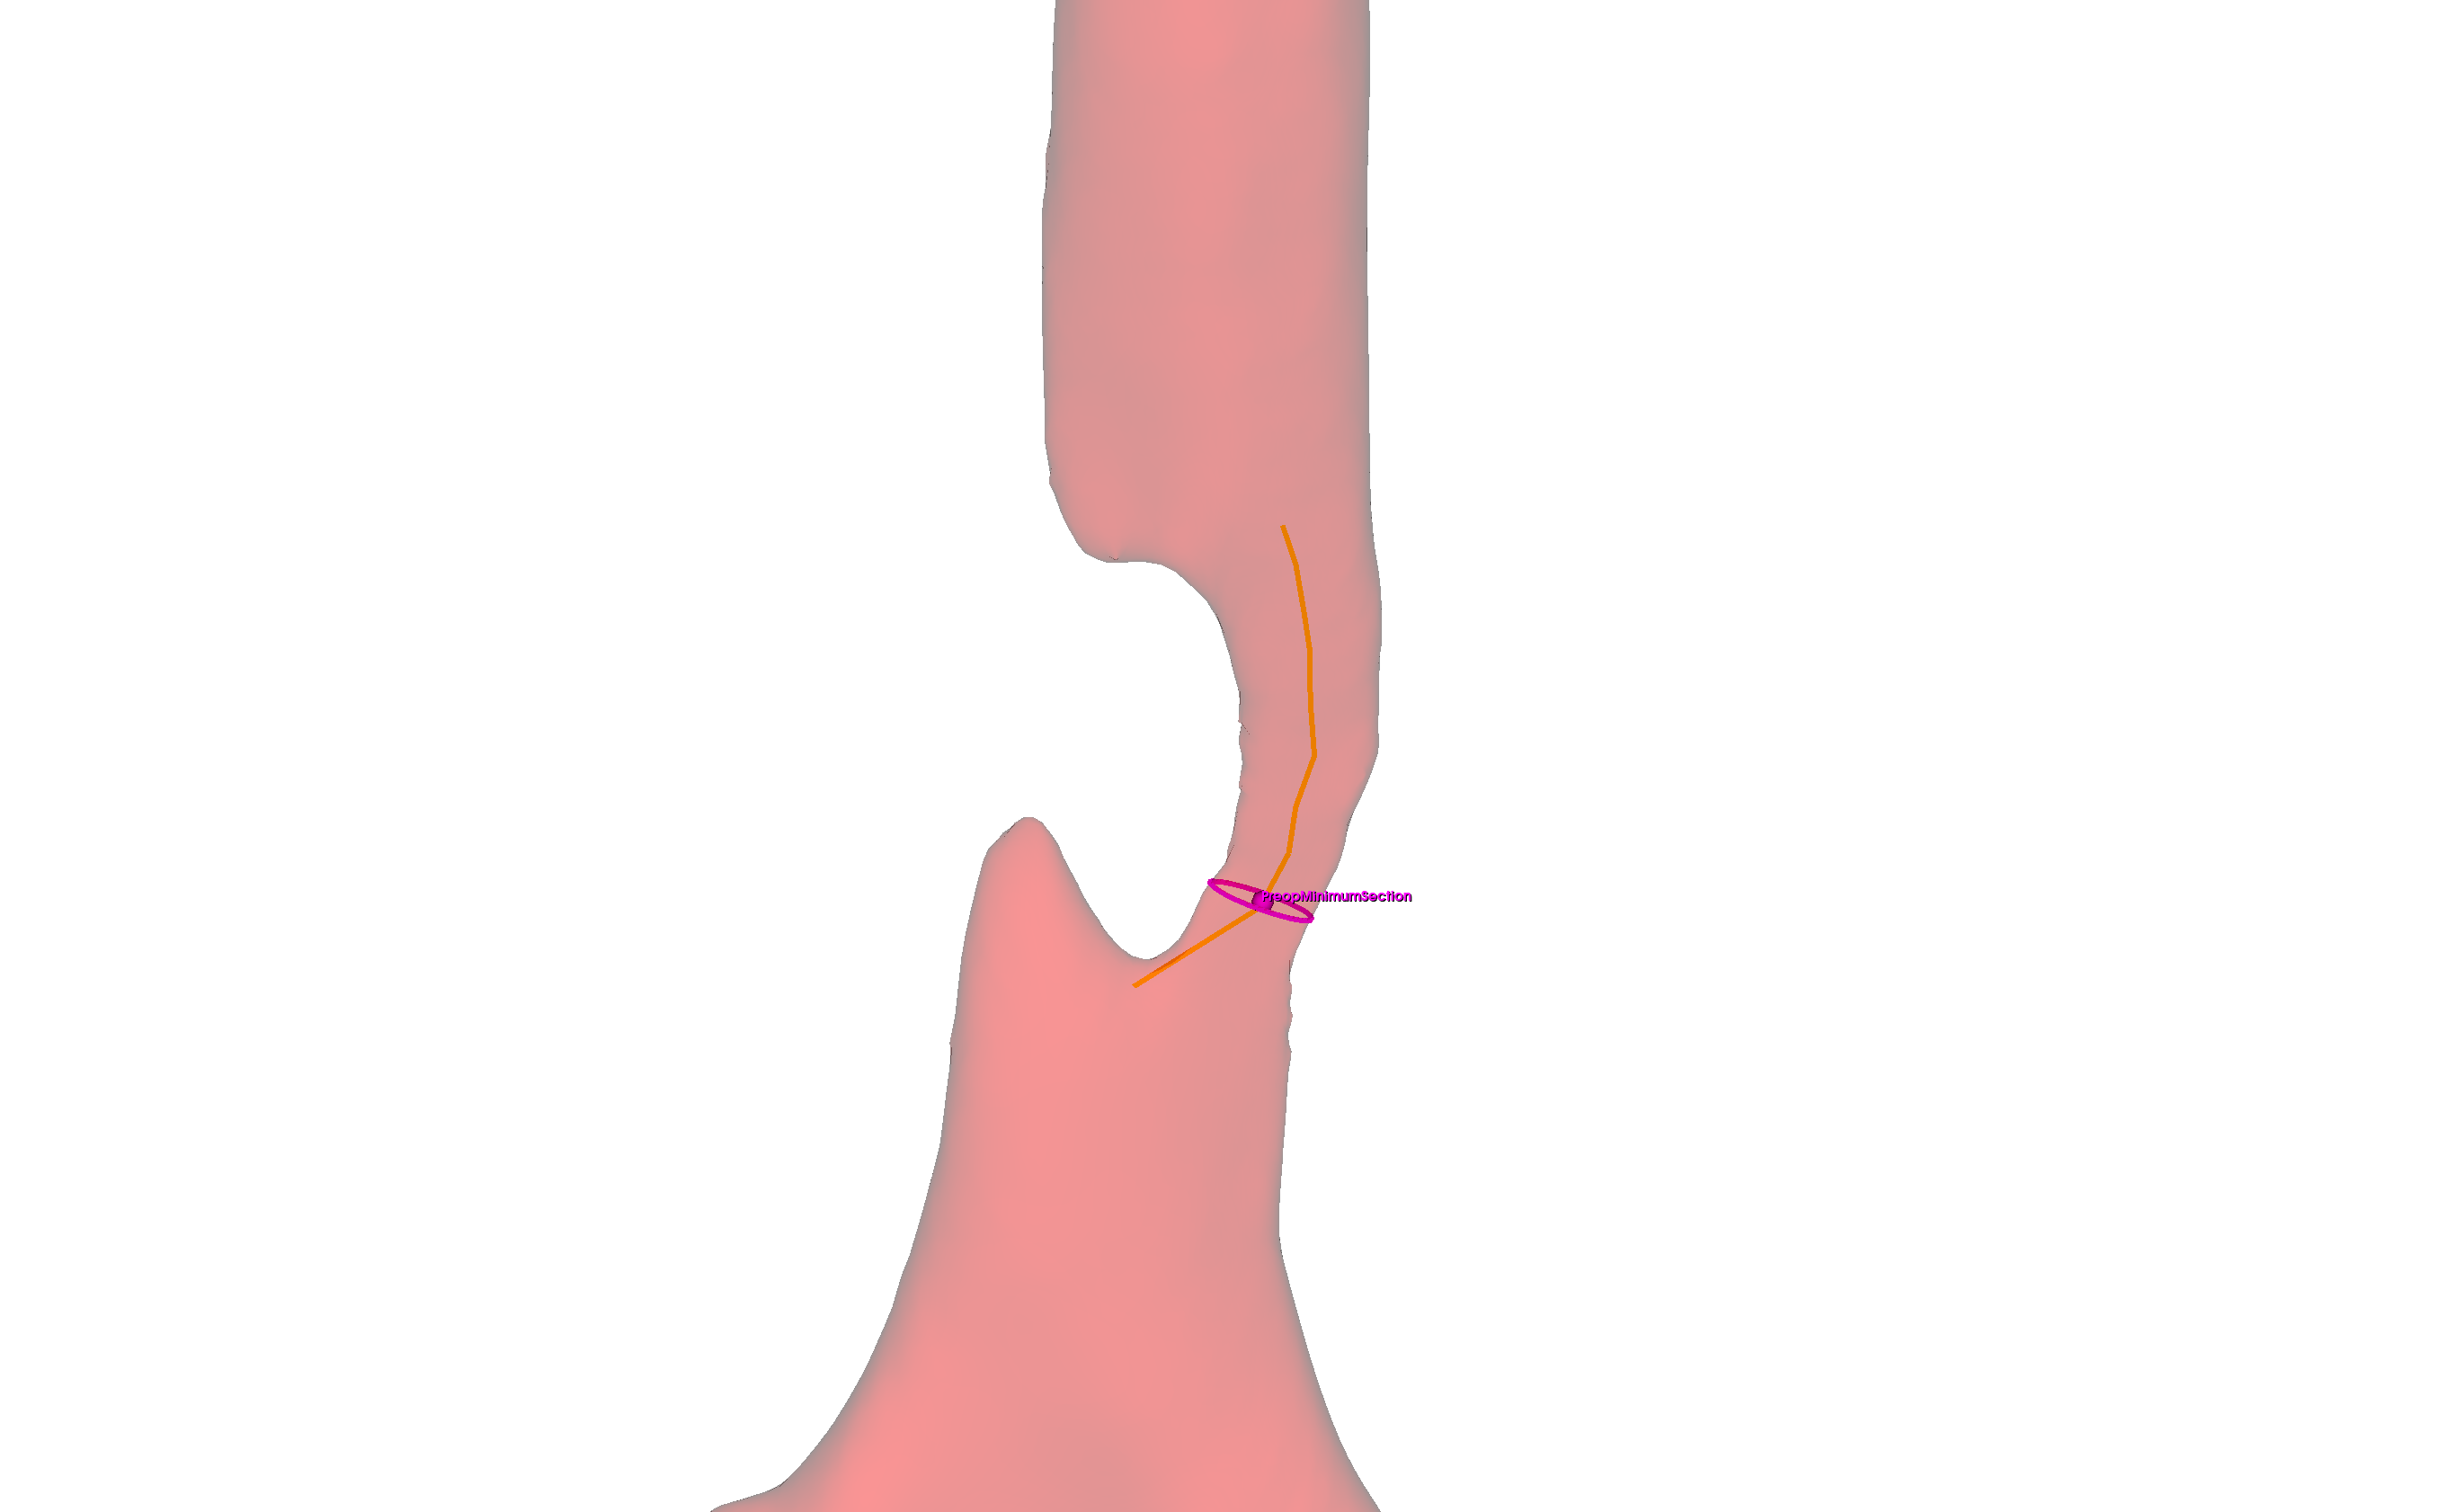
\includegraphics[width=\linewidth,height=0.62\textheight,keepaspectratio]{preop_stenosis_measurement.png}
  \end{columns}
\end{frame}

\begin{frame}{Reproducible workflow}
  \centering
  \large
  \begin{block}{Image to result}
    DICOM $\rightarrow$ 3D Slicer/SlicerVMTK $\rightarrow$ capped STL
    $\rightarrow$ Gmsh $\rightarrow$ OpenFOAM $\rightarrow$ ParaView
  \end{block}
  \vspace{0.5em}
  \begin{columns}[T,onlytextwidth]
    \column{0.48\textwidth}
      \textbf{Geometry preparation}
      \begin{itemize}
        \item Case-specific airway segmentation
        \item Centerline-normal measurements
        \item Centerline-directed extensions and planar caps
      \end{itemize}
    \column{0.48\textwidth}
      \textbf{Flow solution}
      \begin{itemize}
        \item Tetrahedral HXT meshes
        \item Steady laminar \texttt{simpleFoam}
        \item Transient postoperative \texttt{pimpleFoam} PoC
      \end{itemize}
  \end{columns}
\end{frame}

\begin{frame}{Patient-specific airway reconstruction}
  \begin{columns}[T,onlytextwidth]
    \column{0.49\textwidth}
      \centering
      \textbf{Preoperative}\par\smallskip
      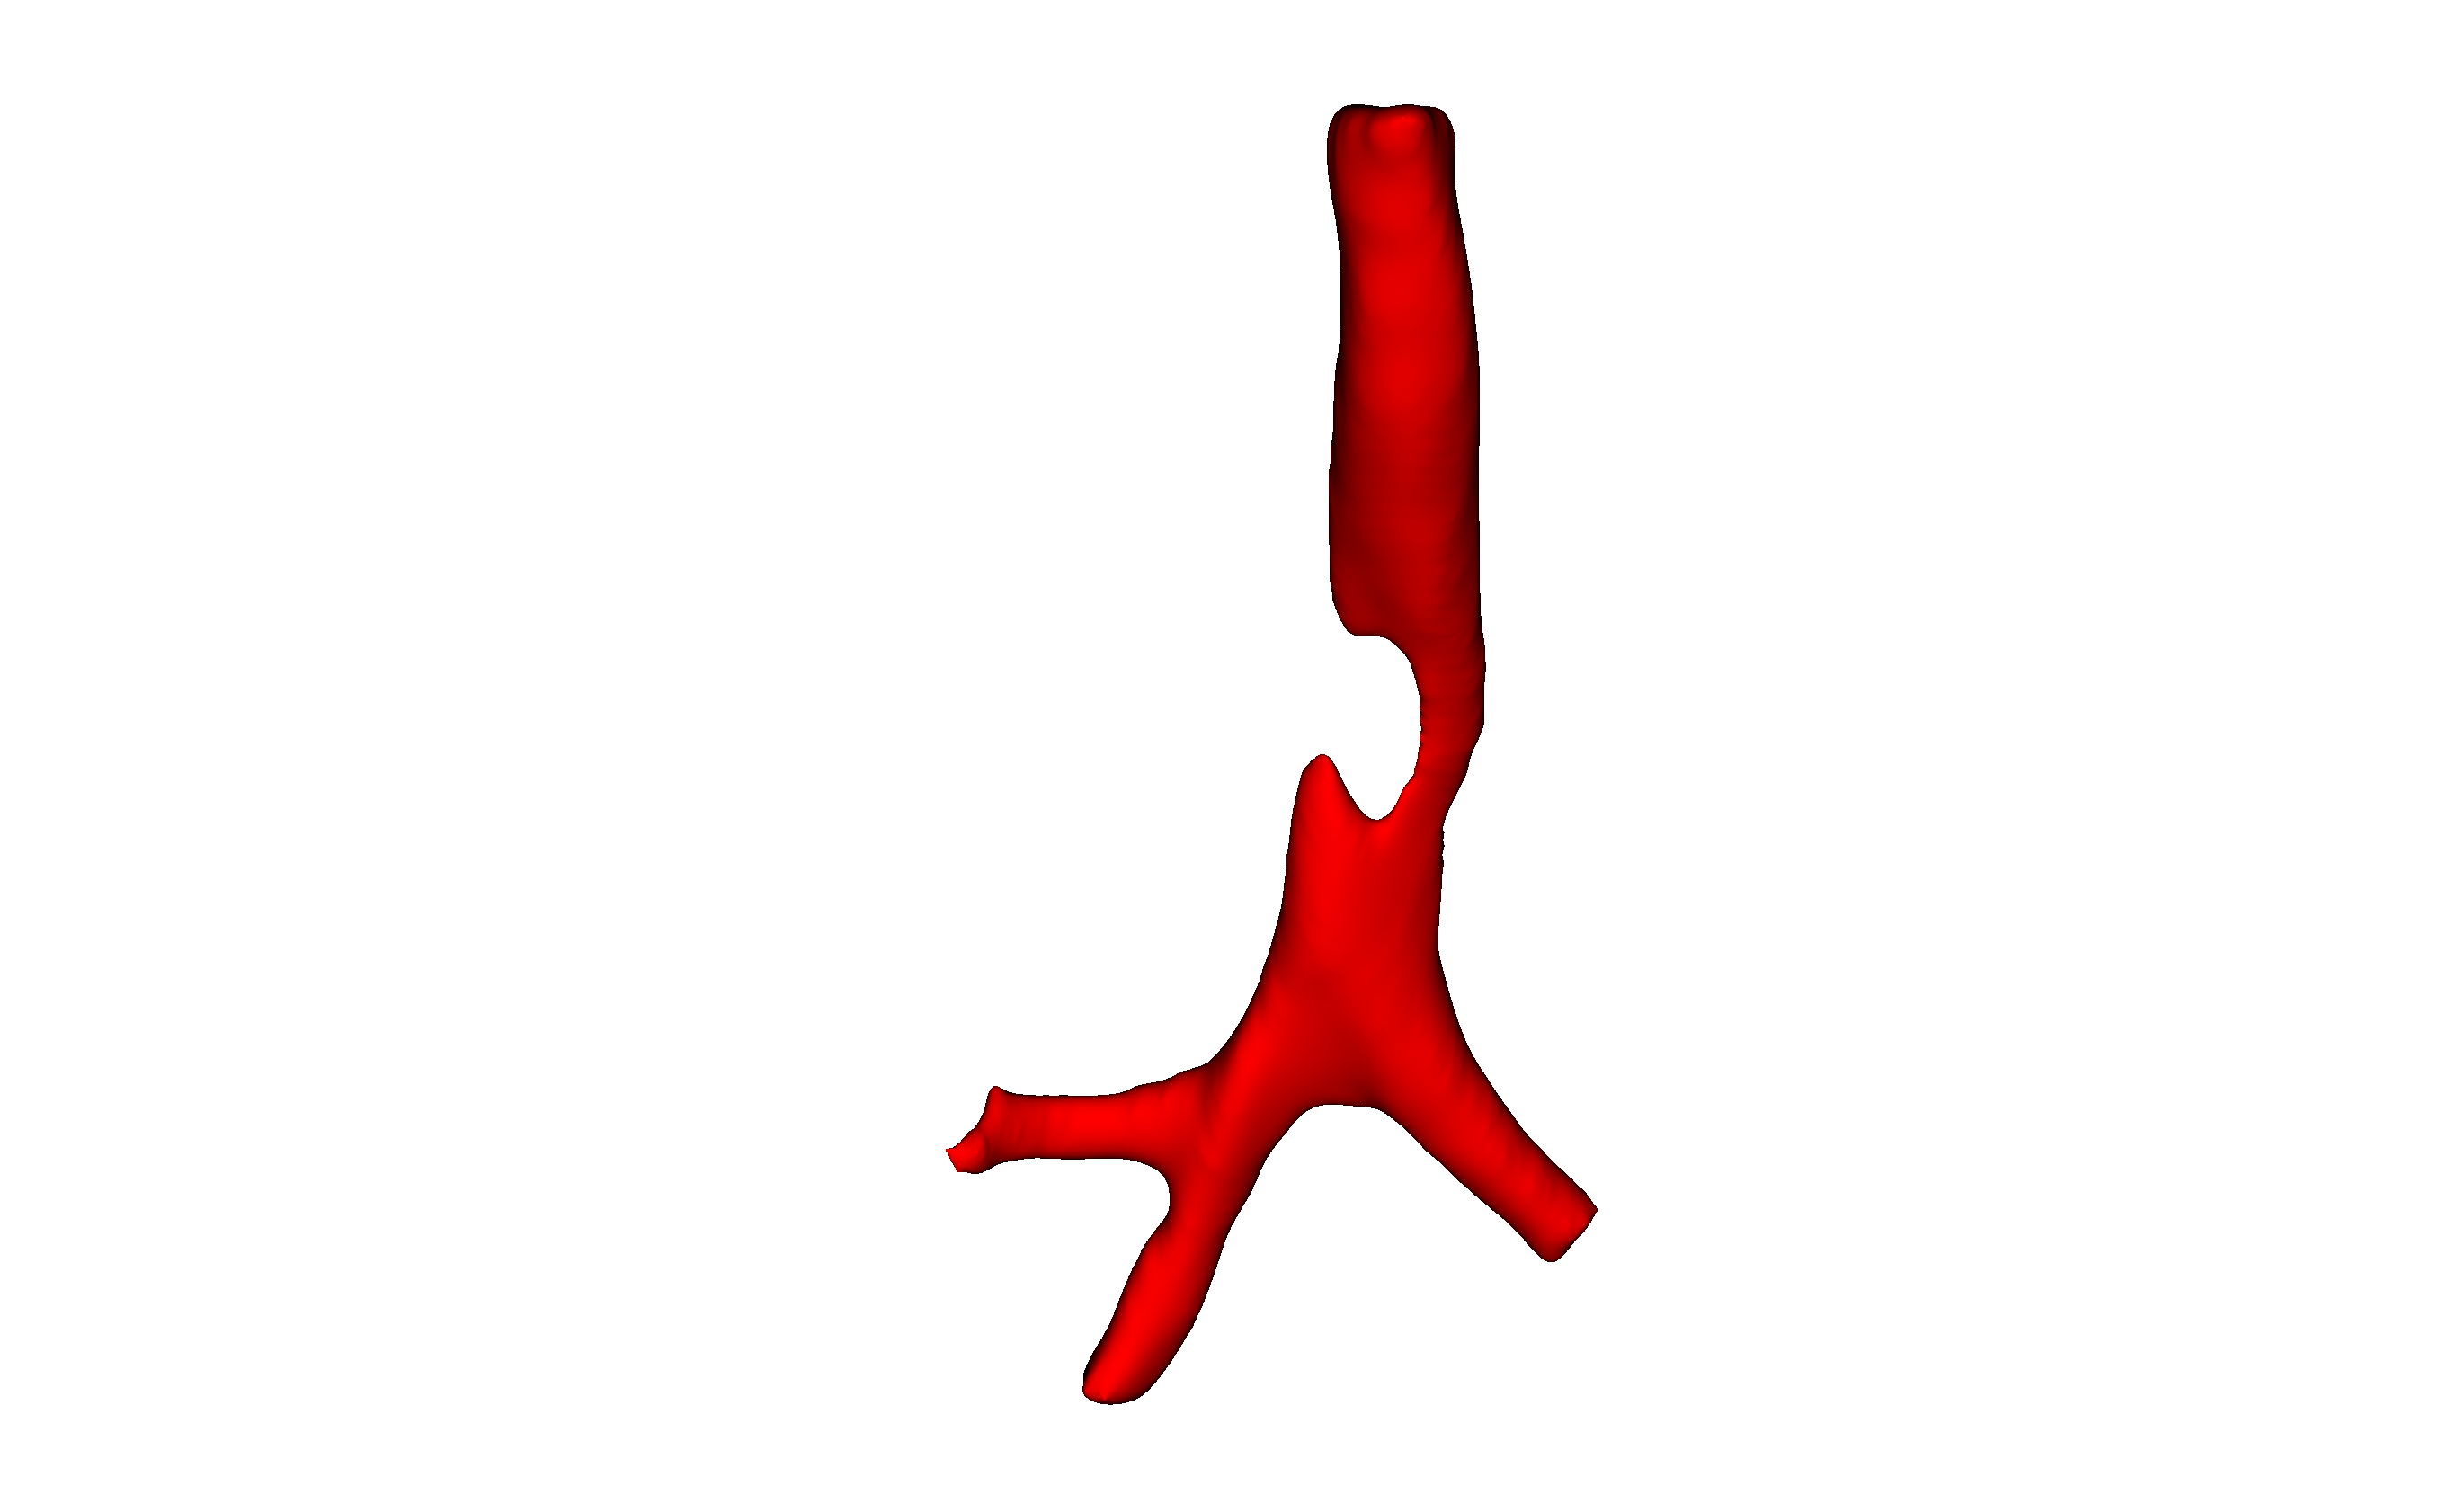
\includegraphics[width=\linewidth,height=0.68\textheight,keepaspectratio]{preop_segmentation.png}
    \column{0.49\textwidth}
      \centering
      \textbf{Postoperative}\par\smallskip
      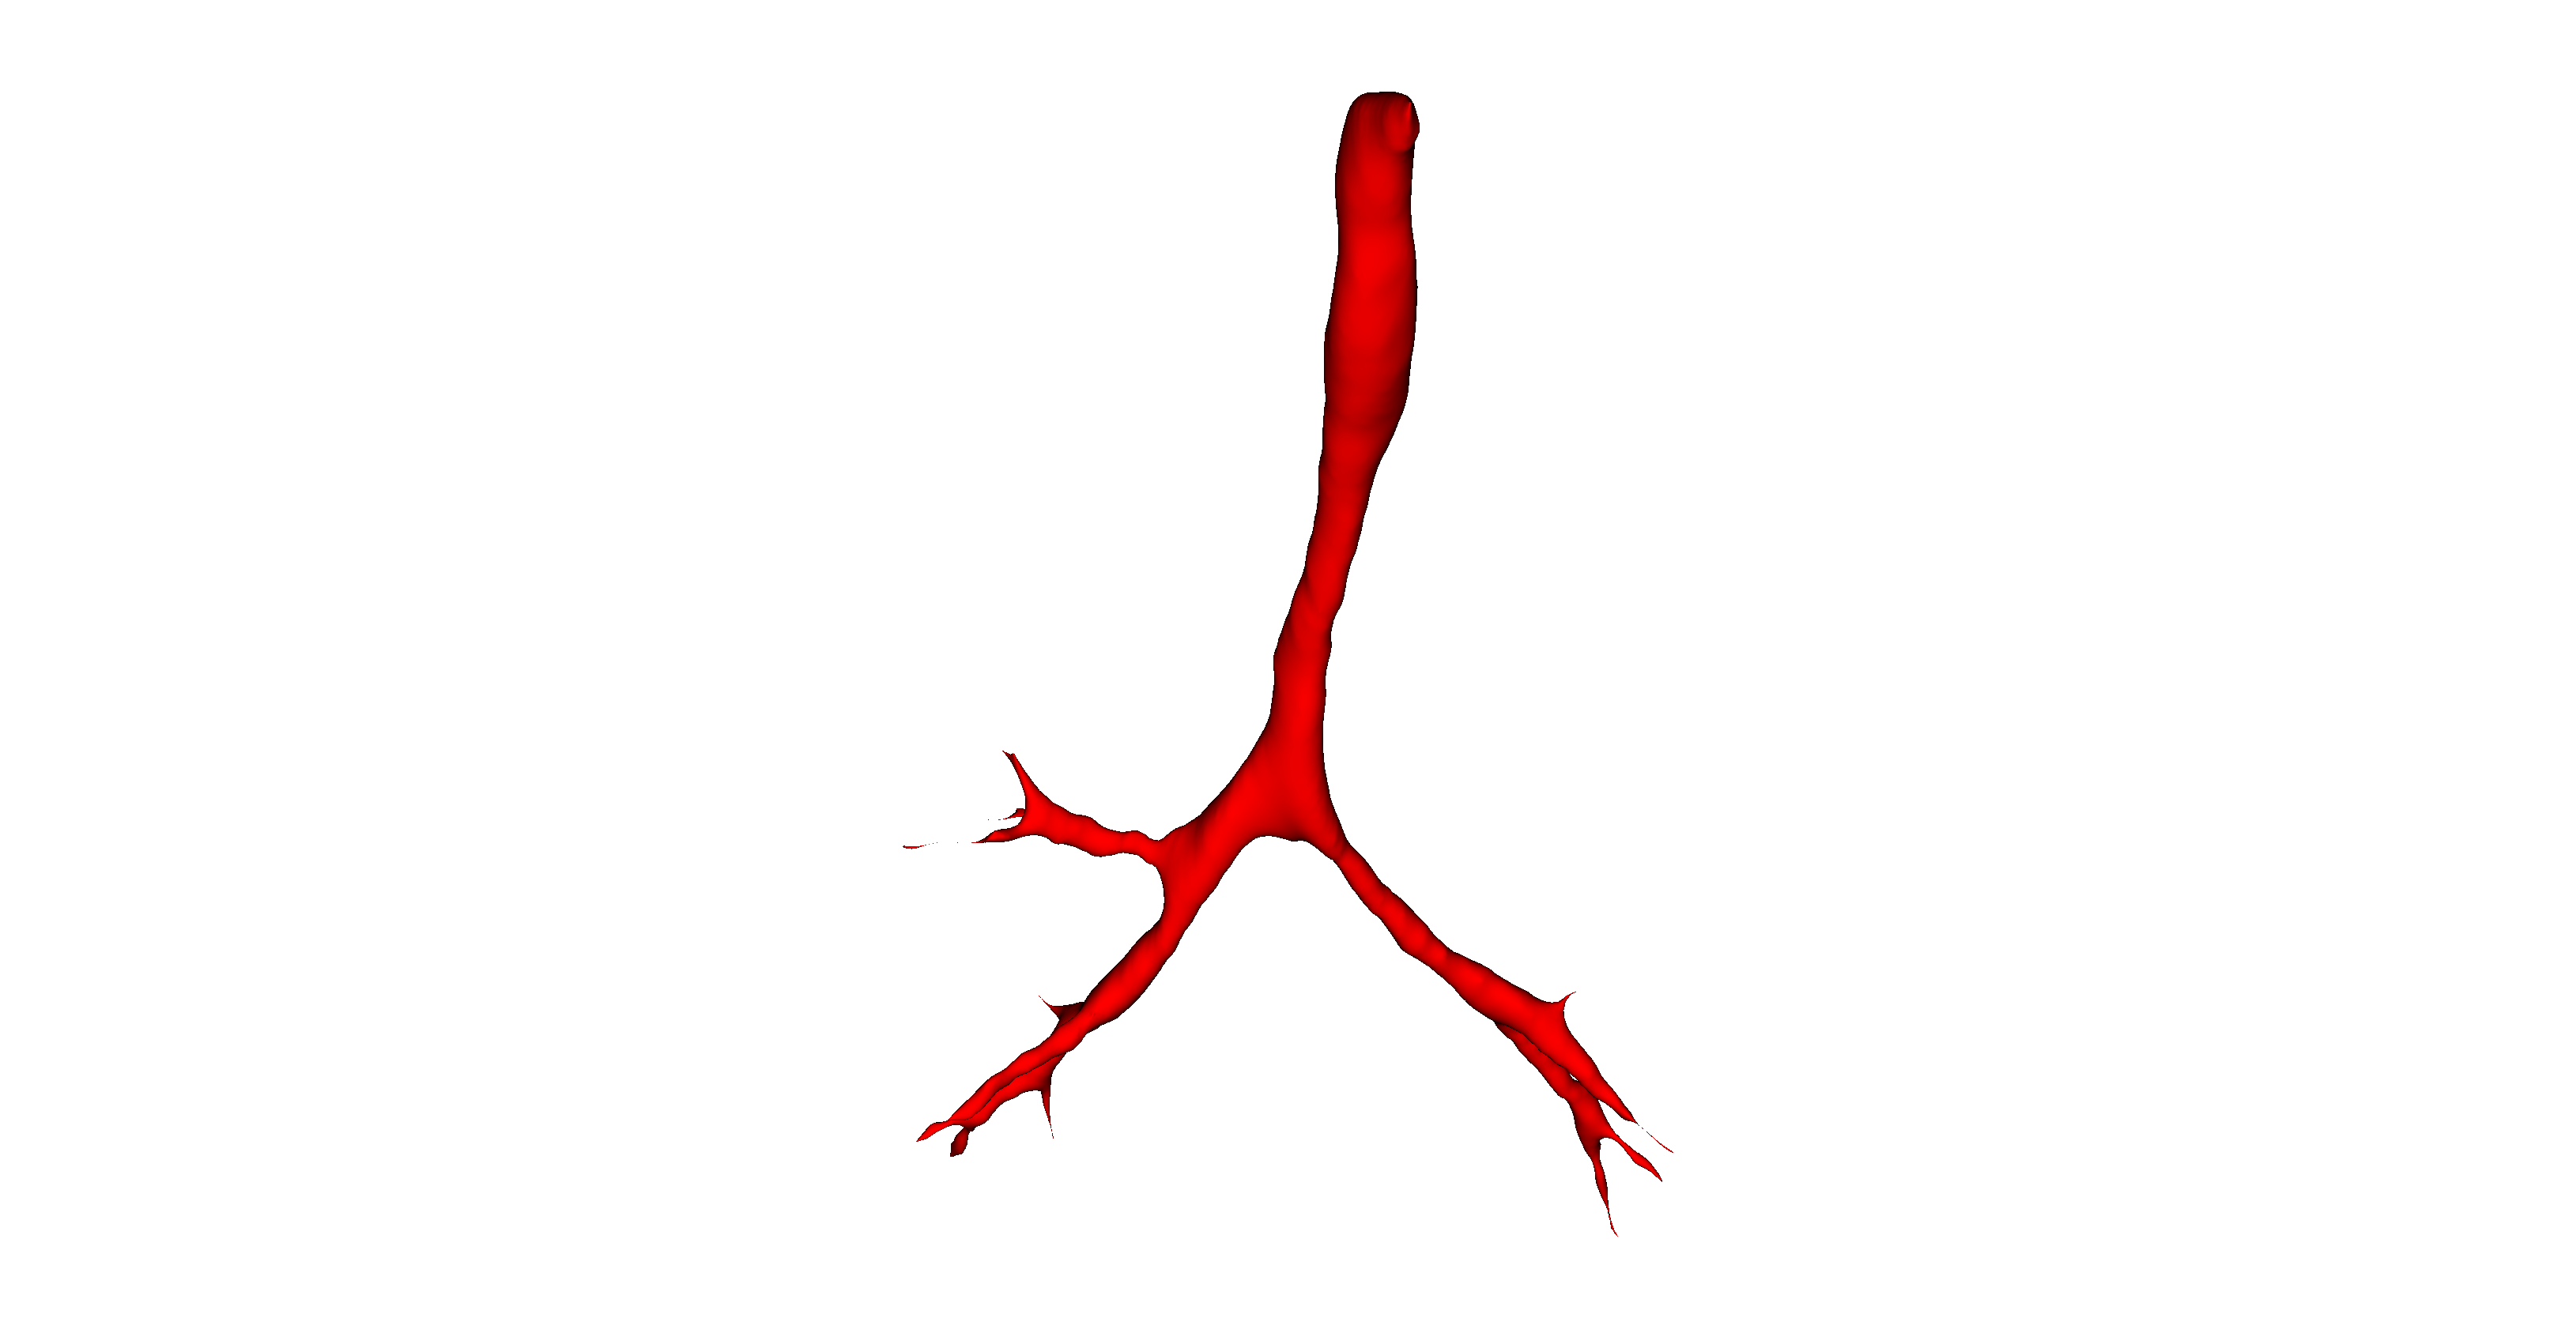
\includegraphics[width=\linewidth,height=0.68\textheight,keepaspectratio]{postop_segmentation.png}
  \end{columns}
  \vspace{-0.2em}
  \centering\small The preoperative stenosis was preserved during segmentation and manually separated from included lung air.
\end{frame}

\begin{frame}{Intervention increased the matched lumen area}
  \begin{columns}[T,onlytextwidth]
    \column{0.47\textwidth}
      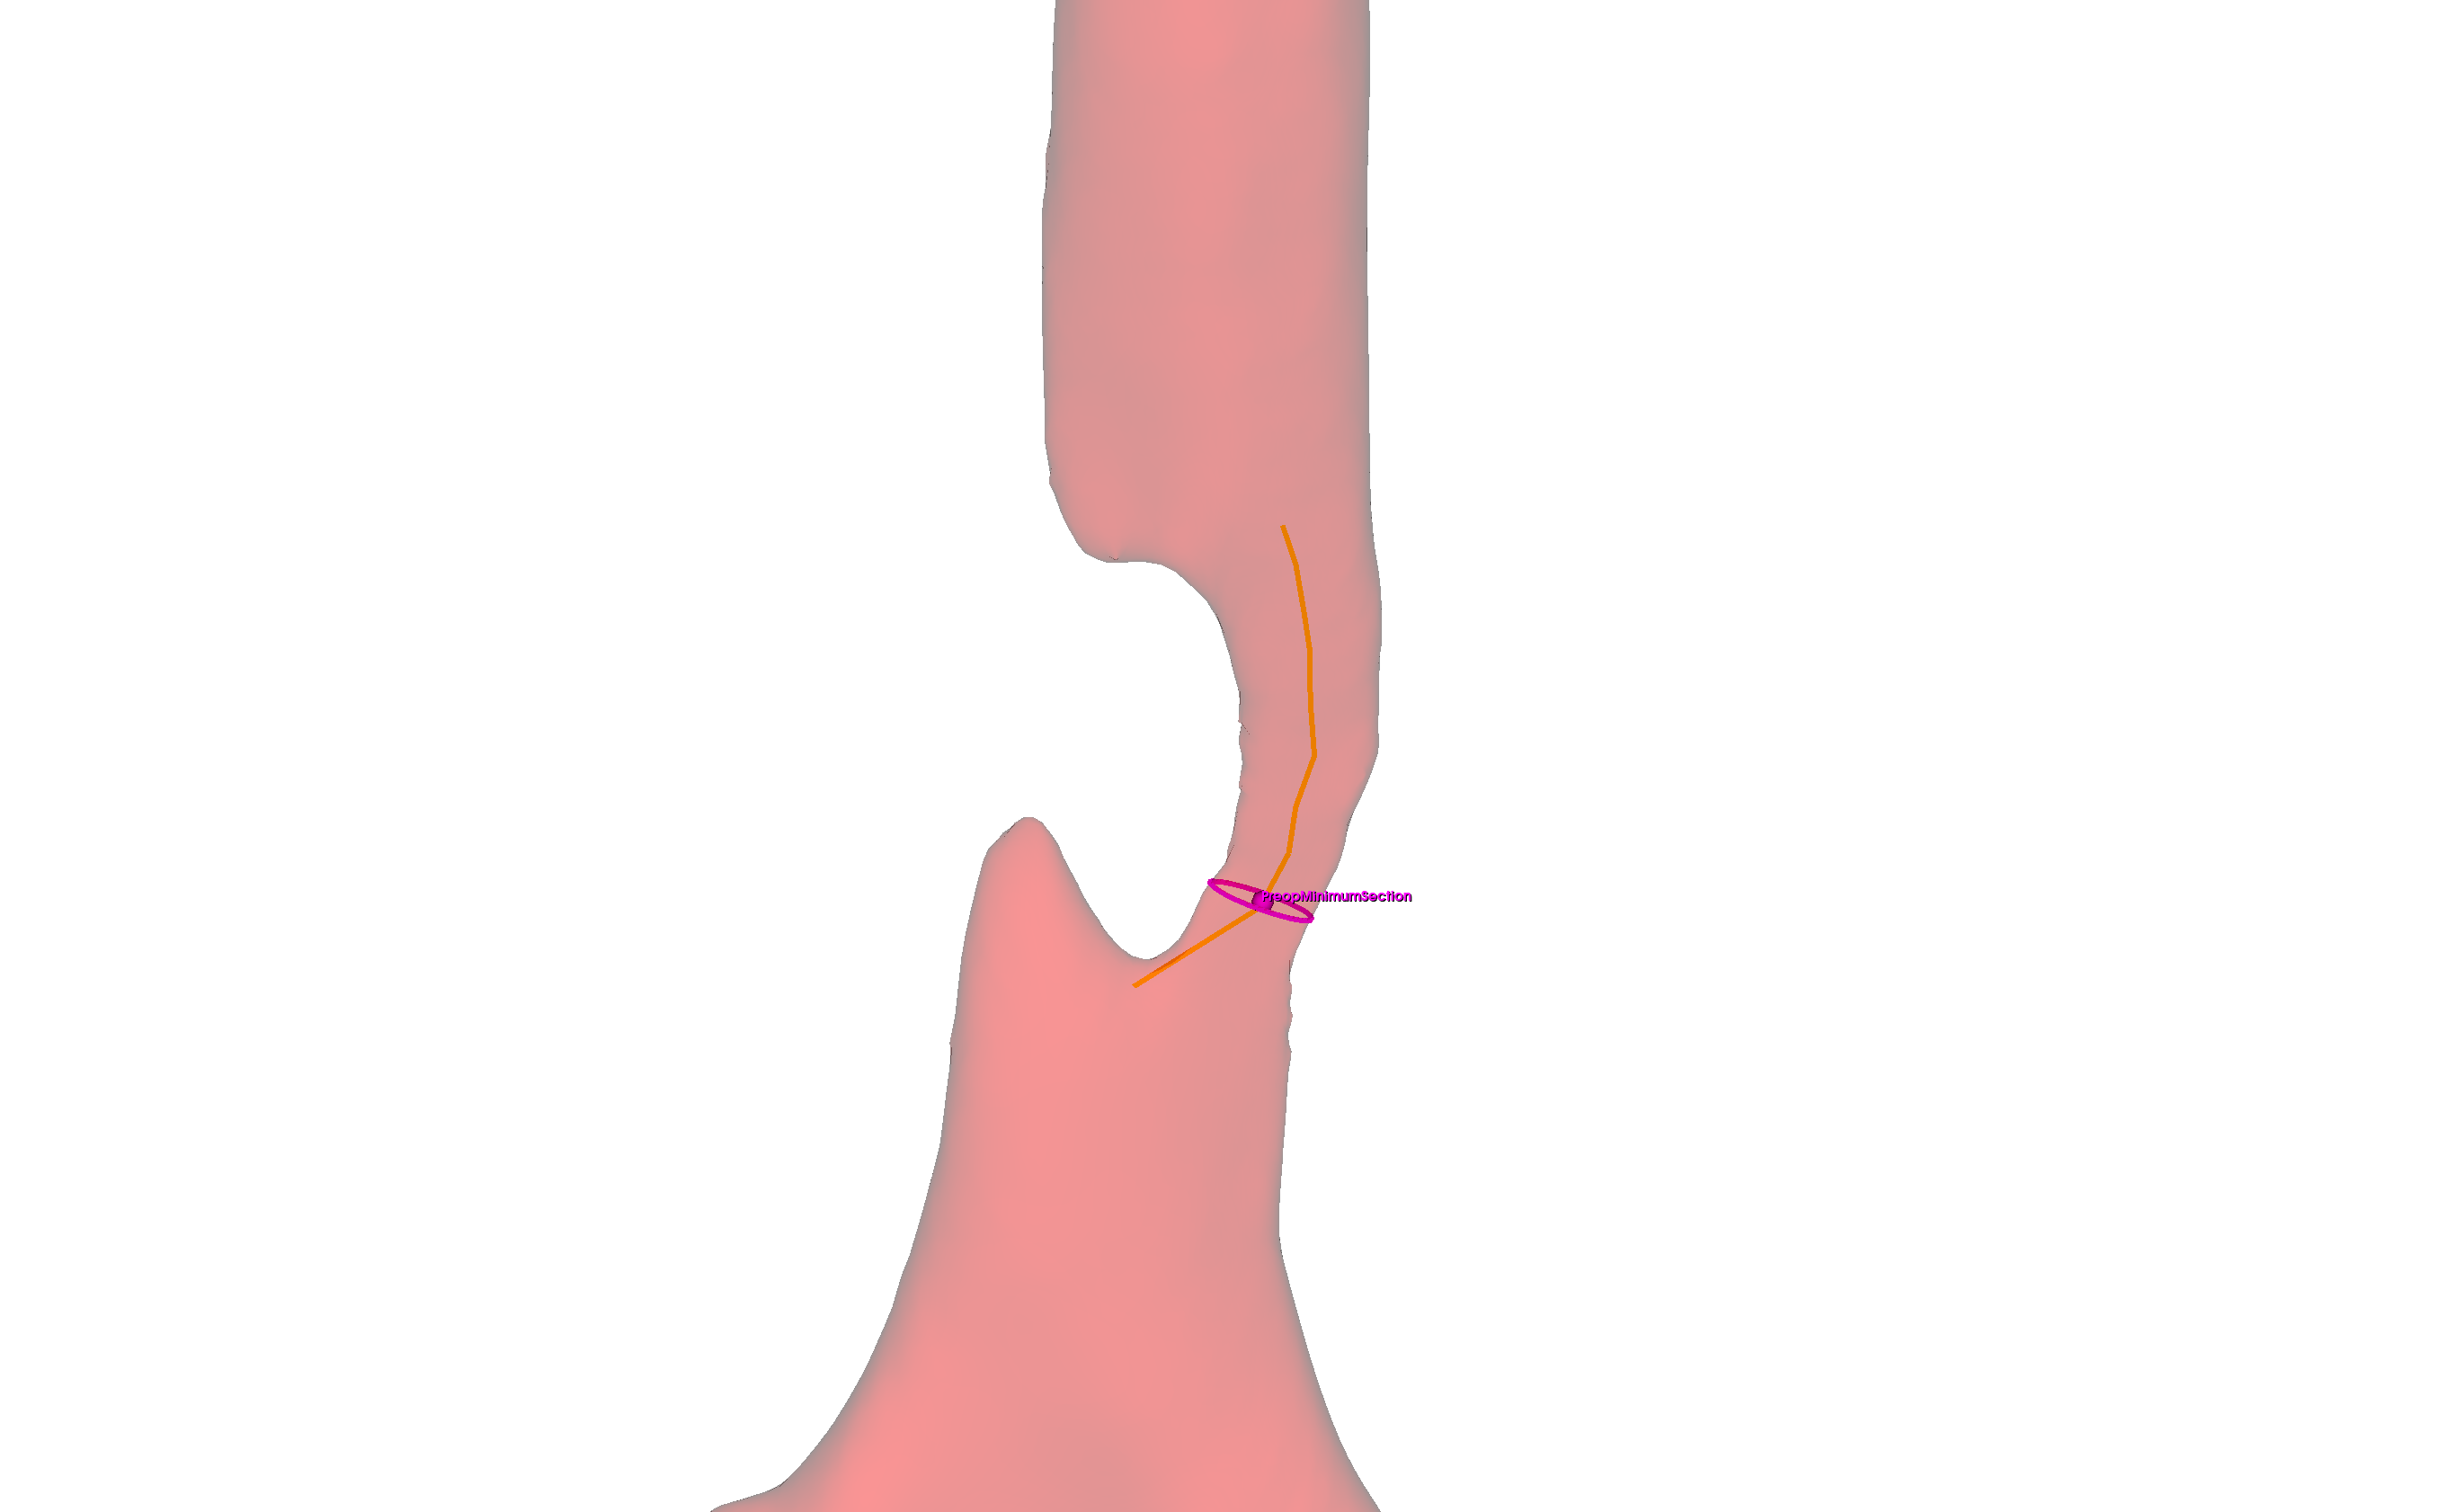
\includegraphics[width=\linewidth,height=0.46\textheight,keepaspectratio]{preop_stenosis_measurement.png}
    \column{0.47\textwidth}
      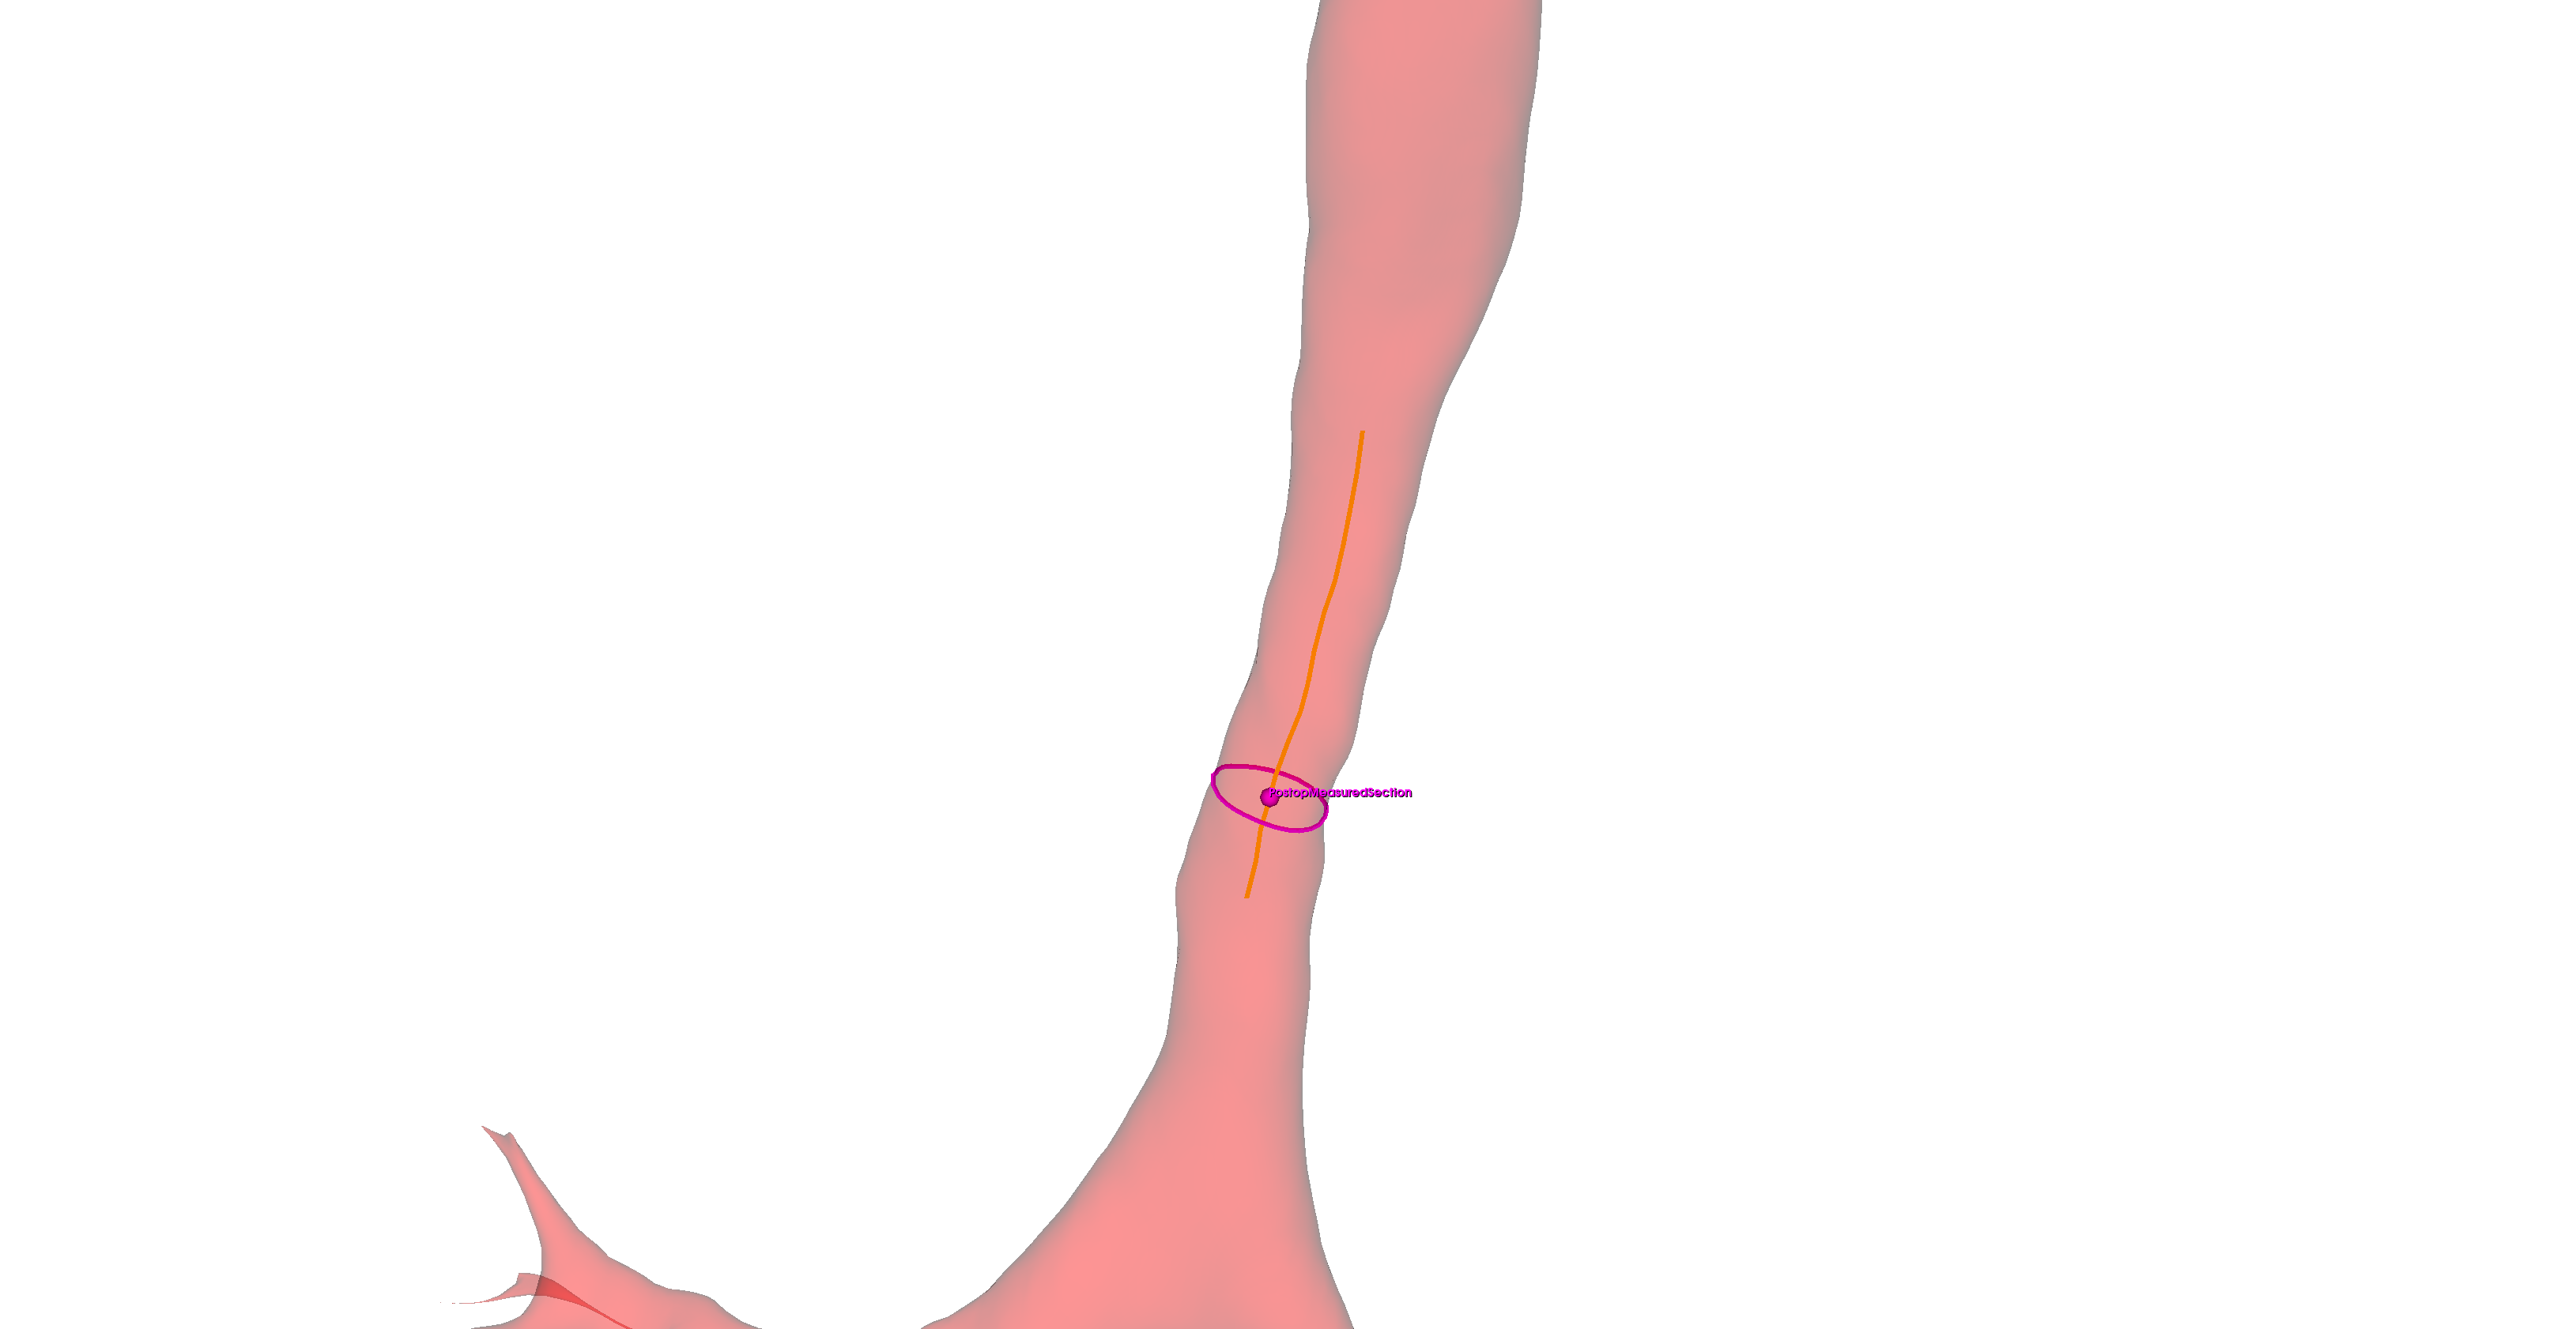
\includegraphics[width=\linewidth,height=0.46\textheight,keepaspectratio]{postop_matched_section.png}
  \end{columns}
  \vspace{-0.2em}
  \begin{center}
    \small
    \begin{tabular}{lrr}
      \toprule
      Quantity & Preoperative & Postoperative \\
      \midrule
      Area (\si{\milli\metre\squared}) & 1.813 & 5.169 \\
      Minimum Feret diameter (\si{\milli\metre}) & 0.798 & 2.292 \\
      Equivalent diameter (\si{\milli\metre}) & 1.519 & 2.565 \\
      \bottomrule
    \end{tabular}
  \end{center}
  \vspace{-0.5em}
  \centering\small\alert{Area constriction: 64.9\%; minimum-Feret reduction: 65.2\%.}
\end{frame}

\begin{frame}{Mesh generation and verification}
  \begin{columns}[T,onlytextwidth]
    \column{0.49\textwidth}
      \centering
      \textbf{0.25 mm baseline}\par\smallskip
      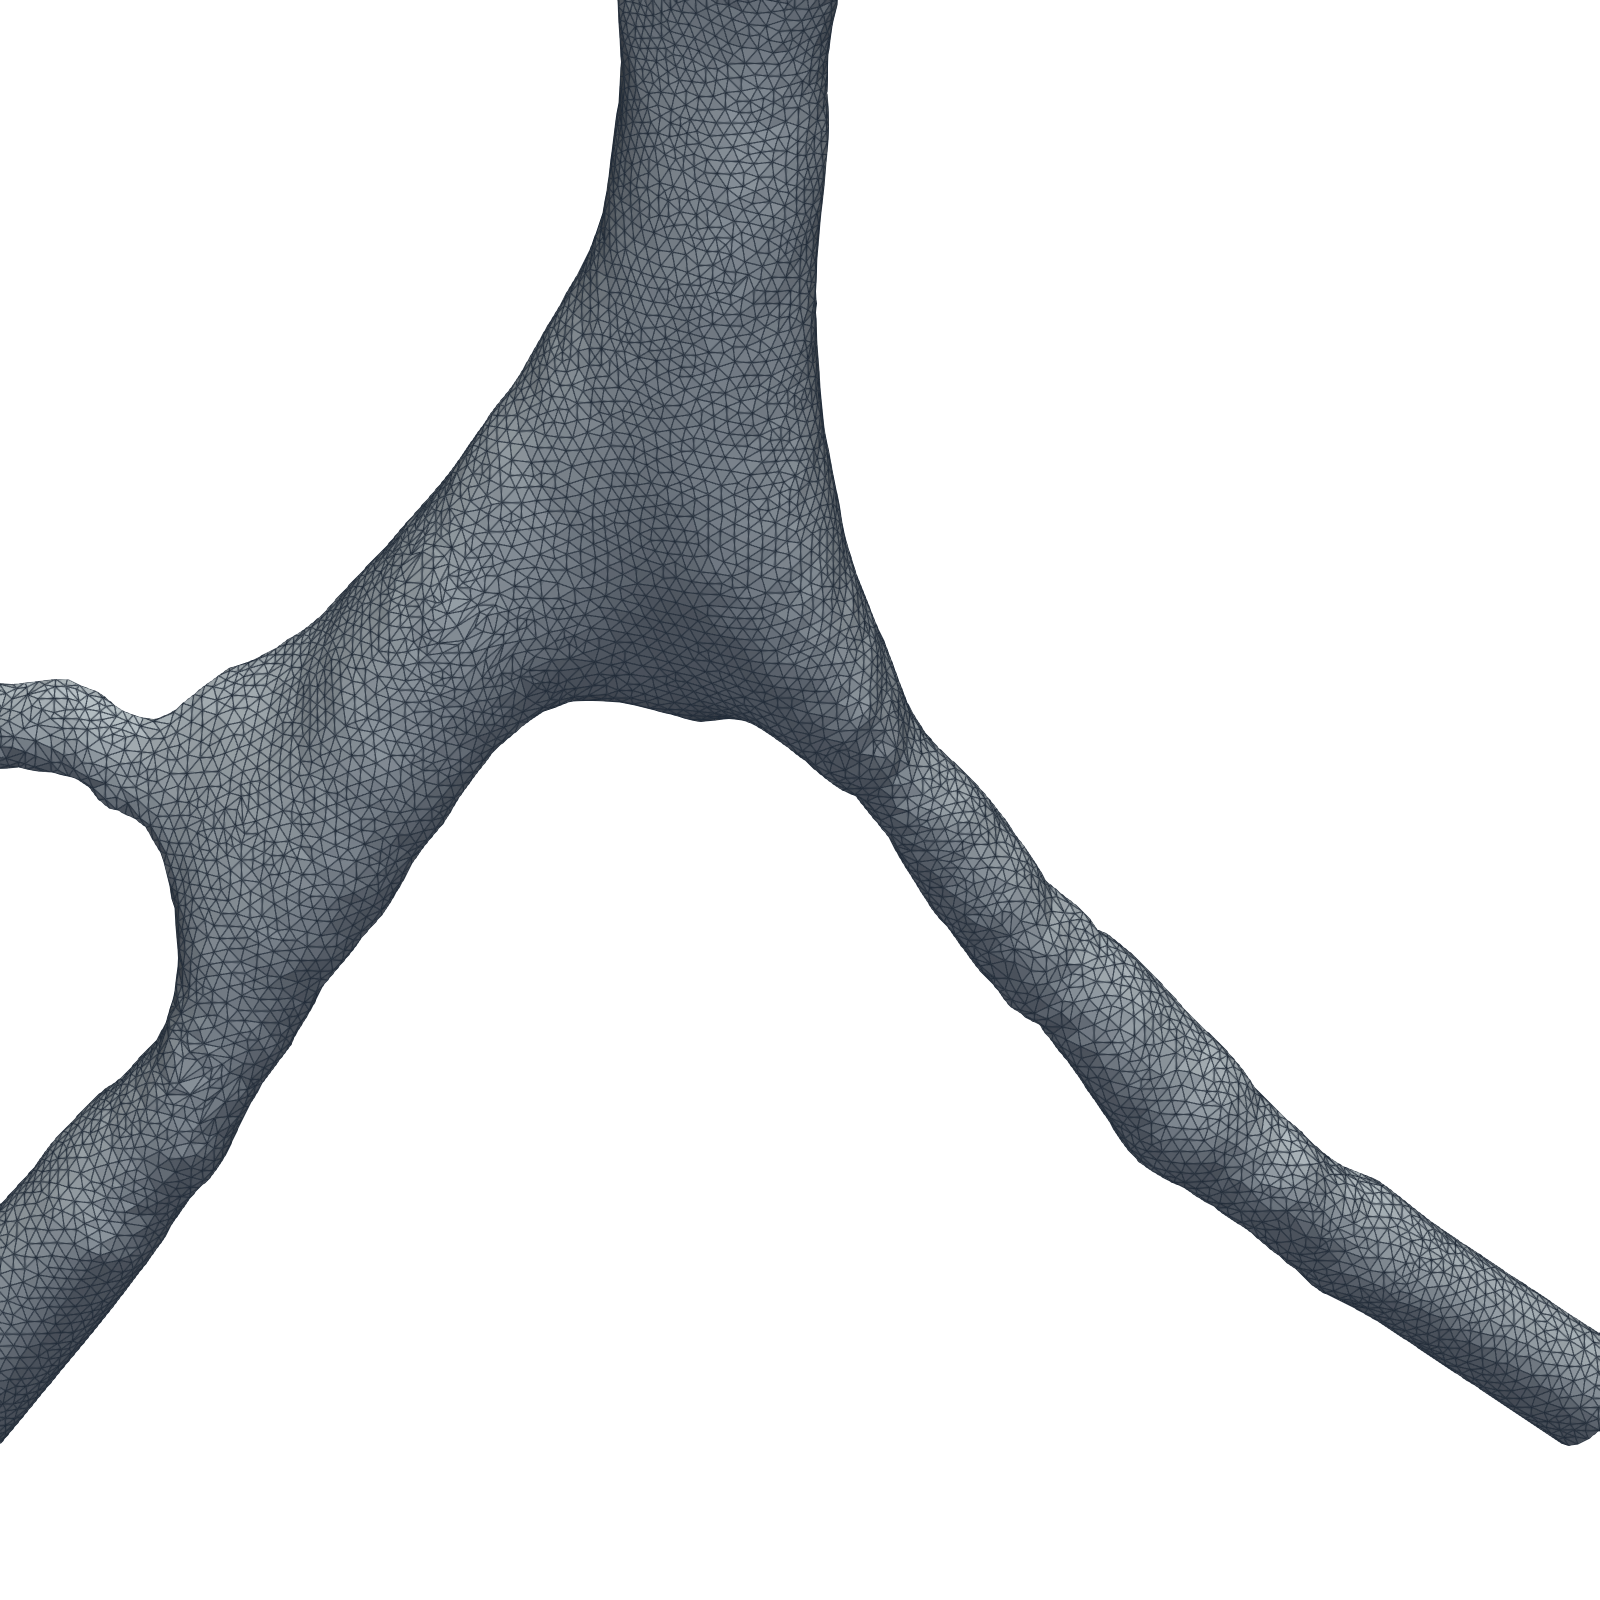
\includegraphics[width=\linewidth,height=0.58\textheight,keepaspectratio]{assignment5_mesh_025_closeup.png}
      \small 180,163 cells
    \column{0.49\textwidth}
      \centering
      \textbf{0.15 mm selected}\par\smallskip
      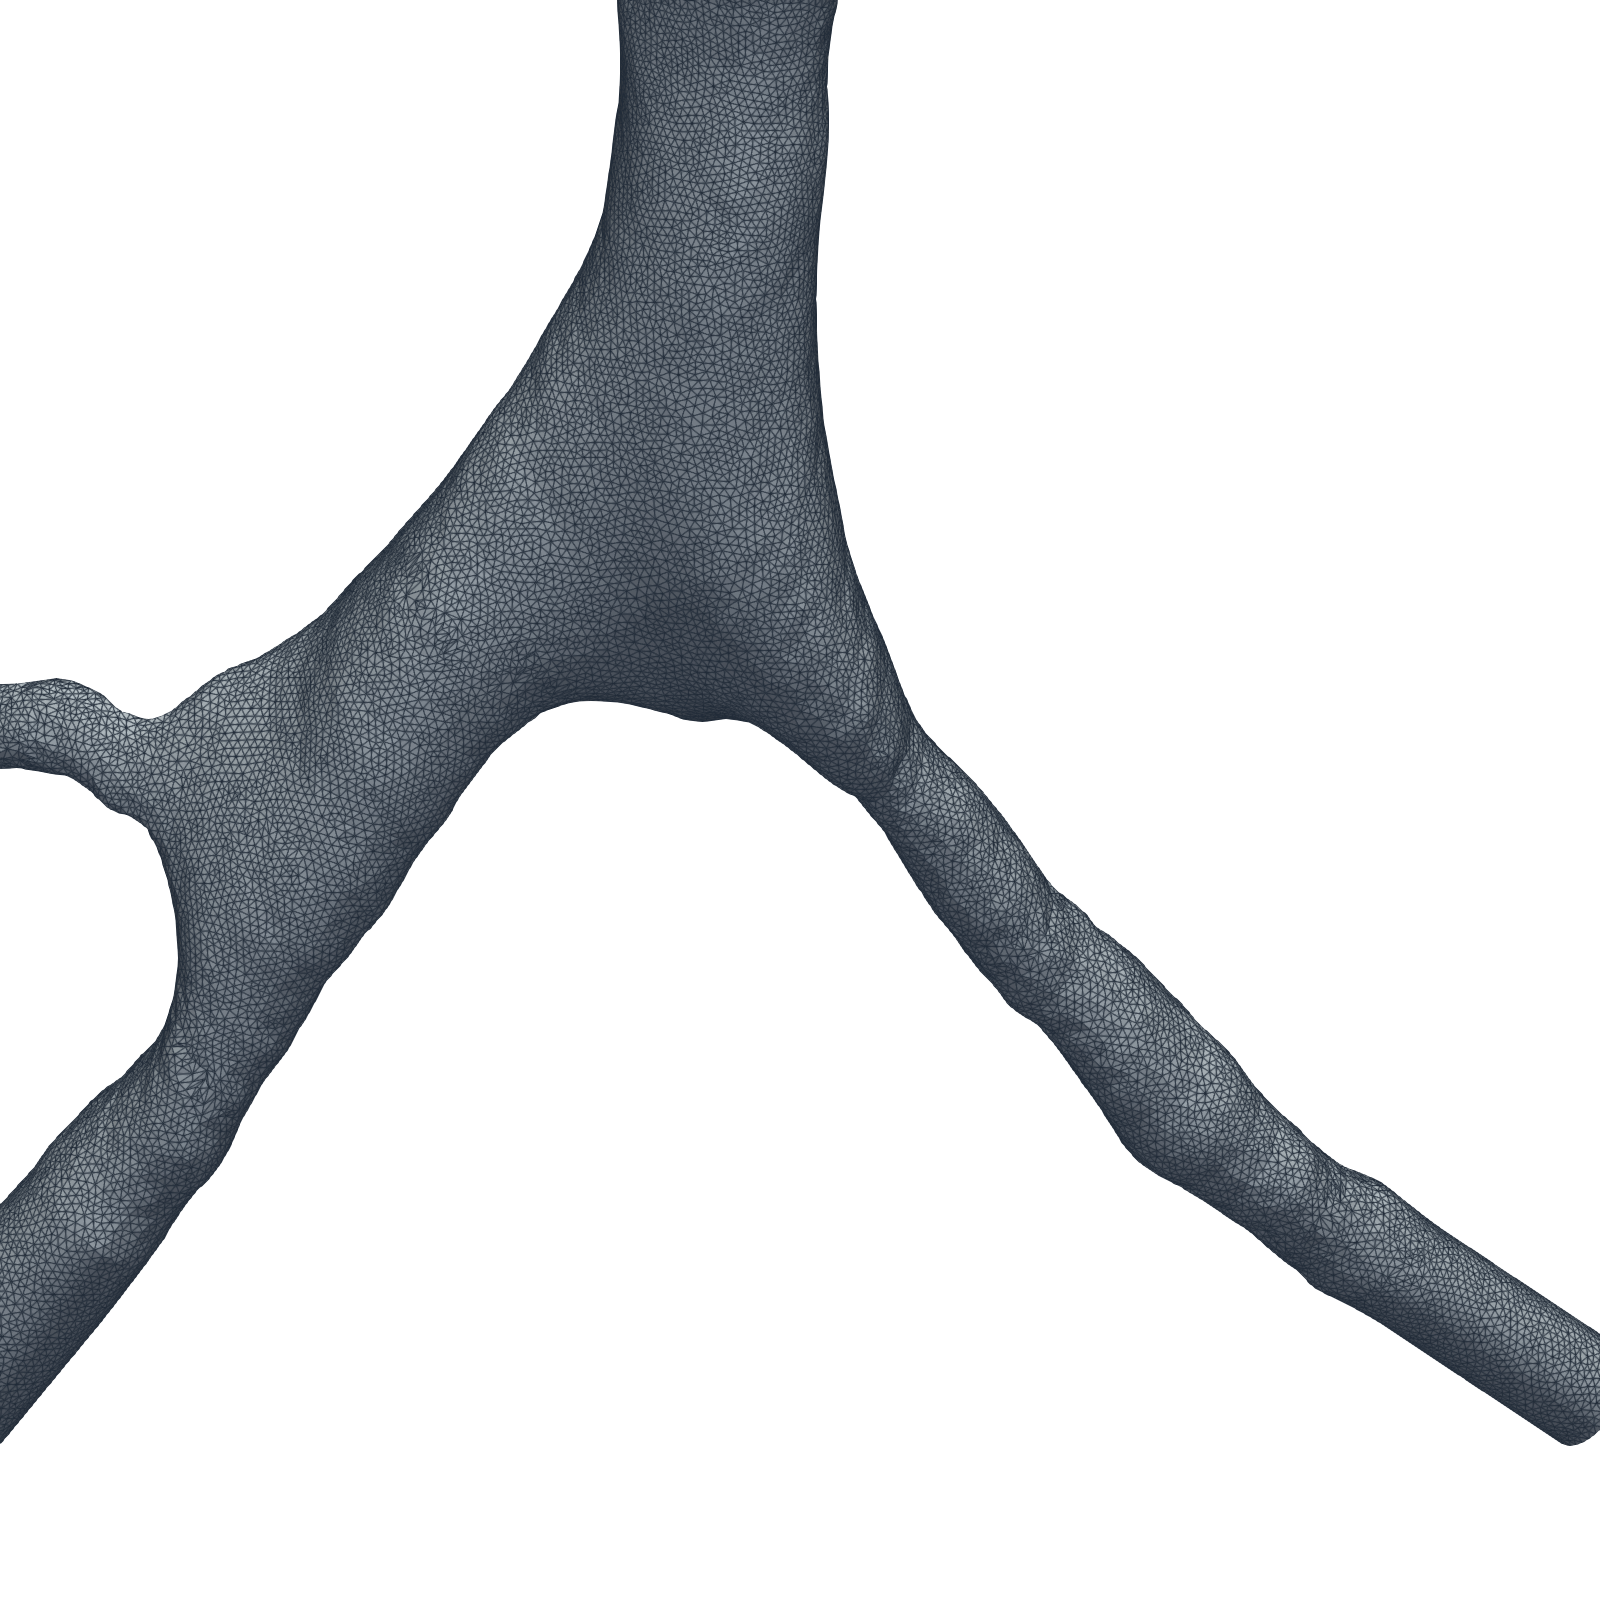
\includegraphics[width=\linewidth,height=0.58\textheight,keepaspectratio]{assignment5_mesh_015_closeup.png}
      \small 776,568 cells
  \end{columns}
  \vspace{0.3em}
  \centering\small The 0.15 mm HXT mesh had no faces above $70^\circ$ non-orthogonality and provided the best accuracy--cost balance.
\end{frame}

\begin{frame}{Mesh sensitivity}
  \centering
  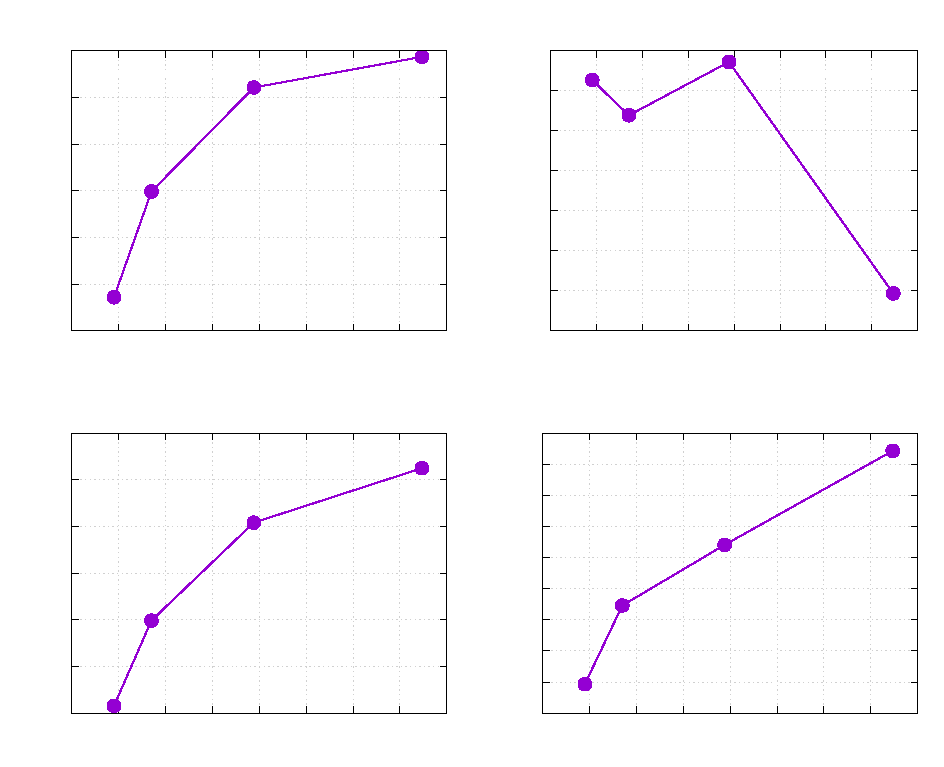
\includegraphics[width=0.86\linewidth,height=0.72\textheight,keepaspectratio]{assignment5_mesh_metrics.pdf}
  \vspace{-0.2em}

  \small From 0.15 to 0.12 mm, selected metrics changed by at most 2.02\%, while cell count increased by 92\% and solver time by 157\%.
\end{frame}

\begin{frame}{Steady postoperative airflow}
  \begin{columns}[T,onlytextwidth]
    \column{0.49\textwidth}
      \centering
      \textbf{Velocity}\par\smallskip
      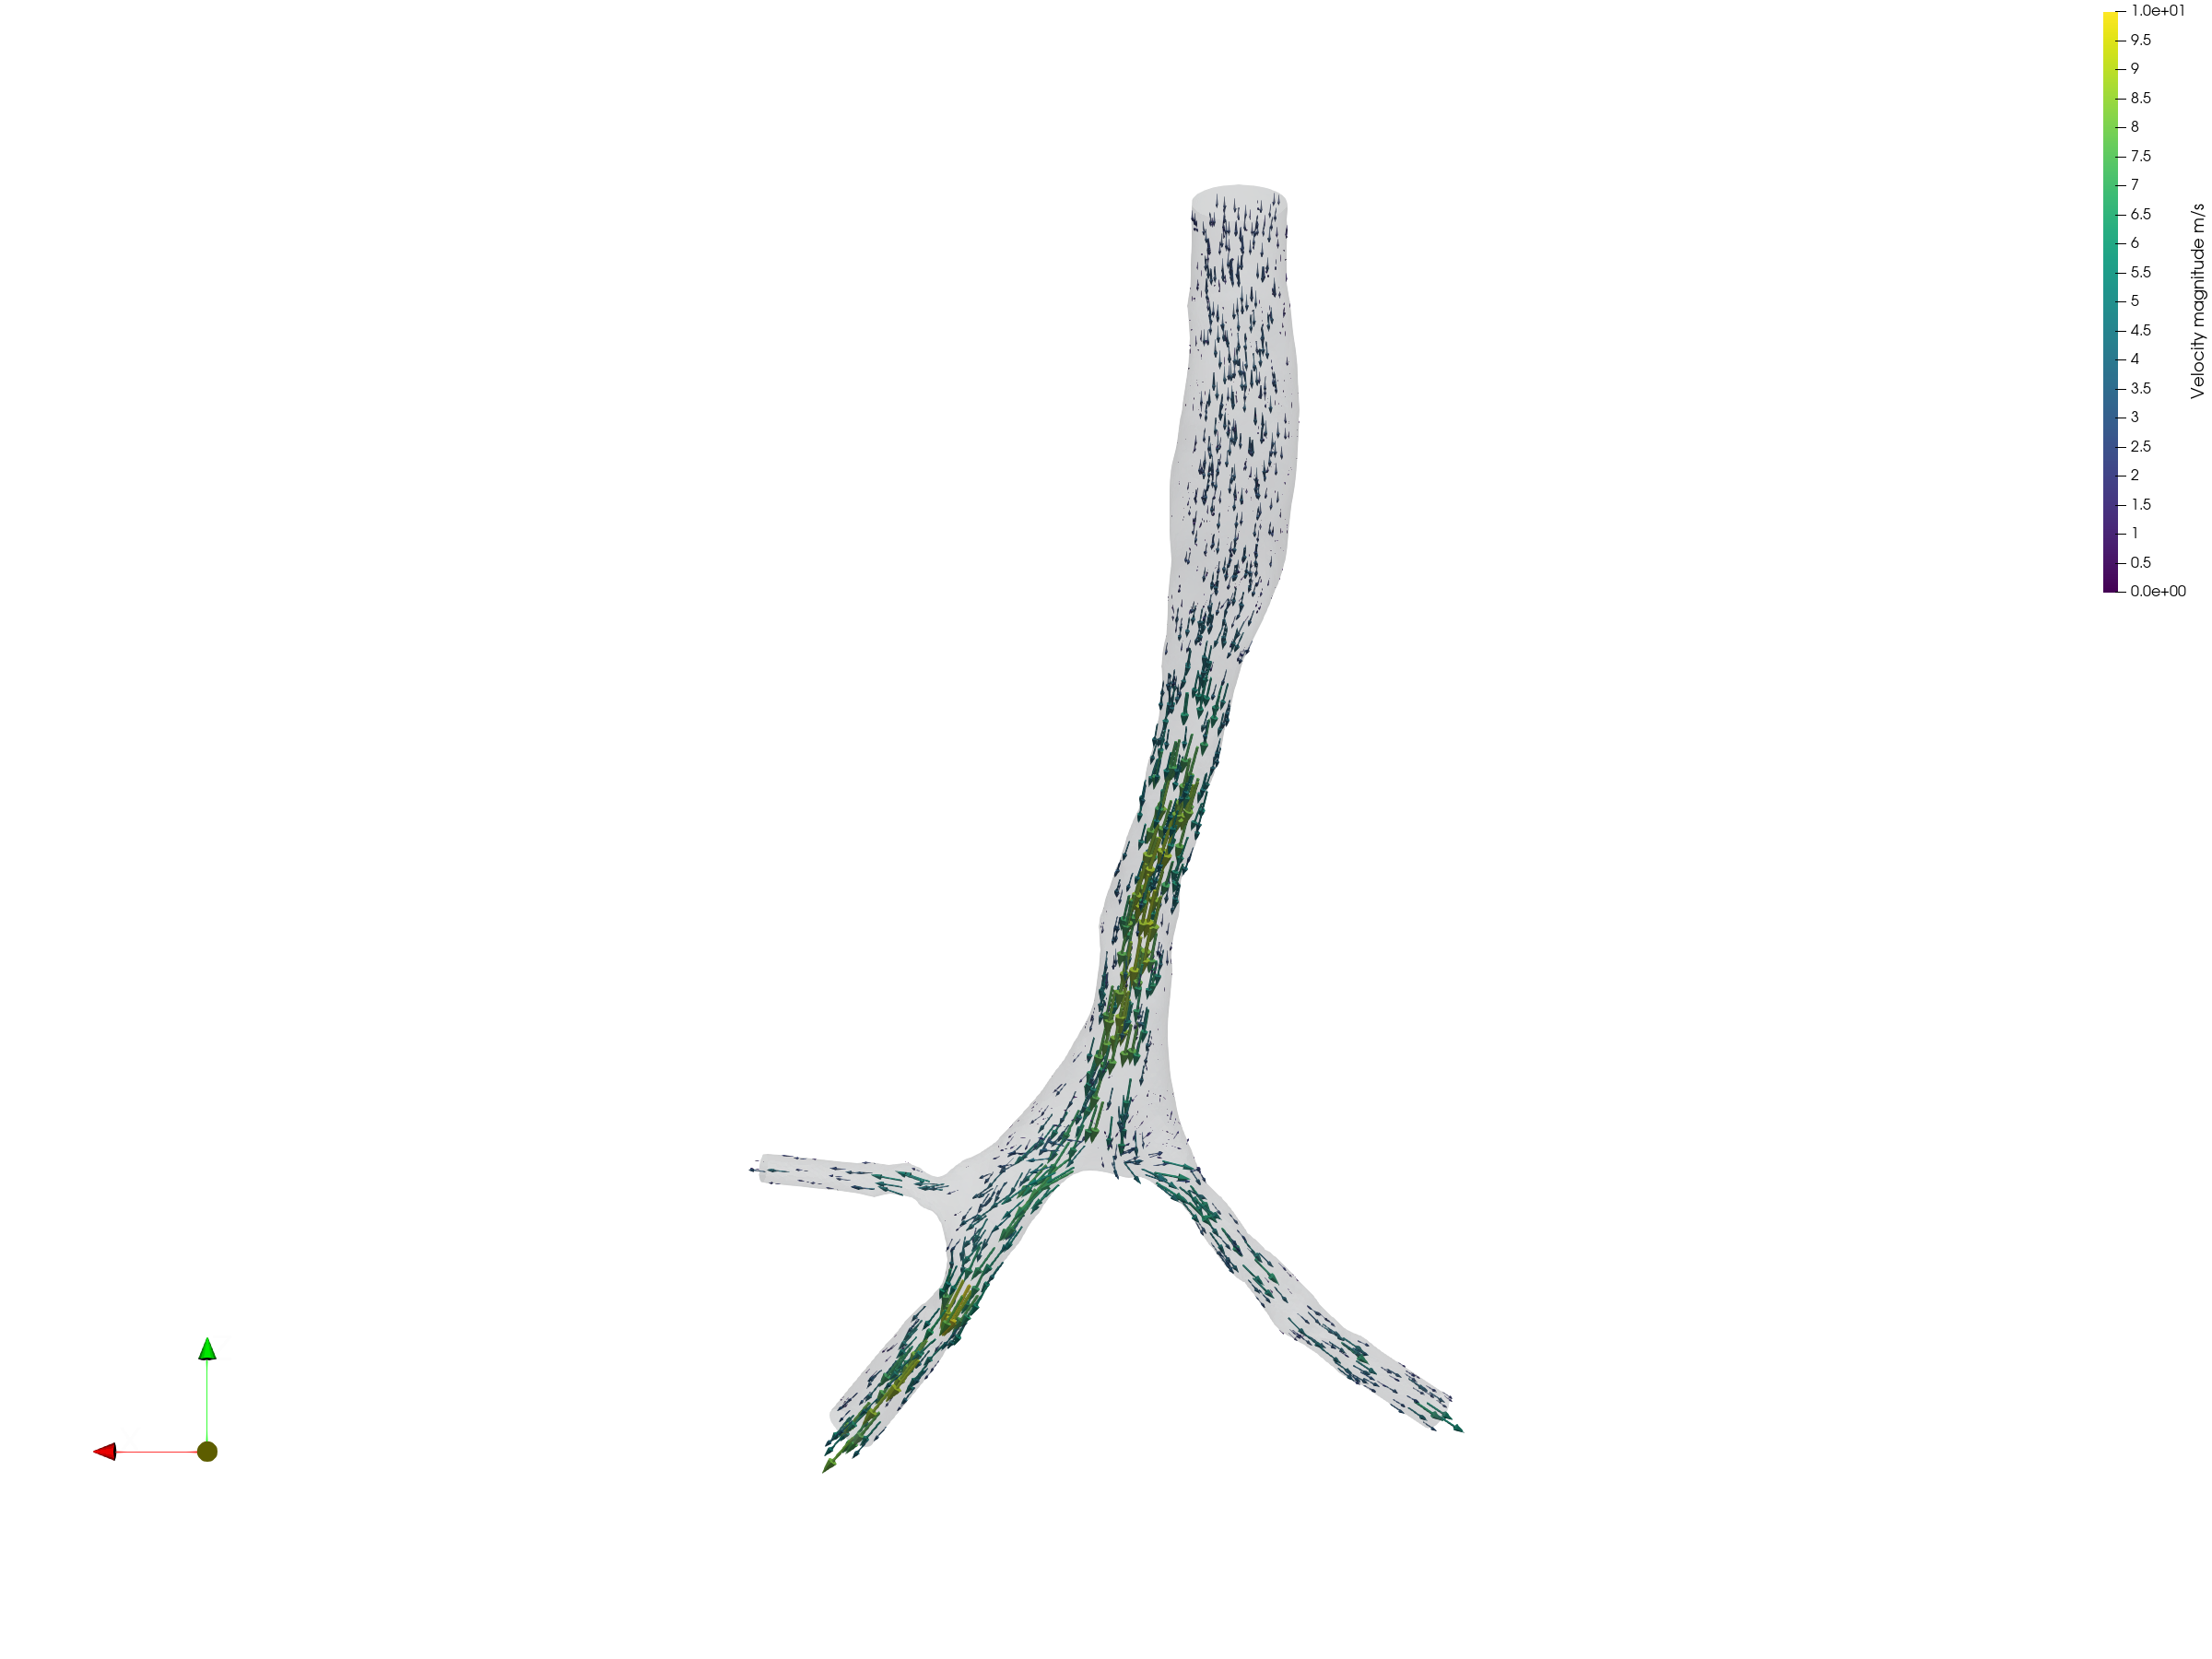
\includegraphics[width=\linewidth,height=0.60\textheight,keepaspectratio]{assignment4_velocity_vectors.png}
    \column{0.49\textwidth}
      \centering
      \textbf{Dimensional pressure}\par\smallskip
      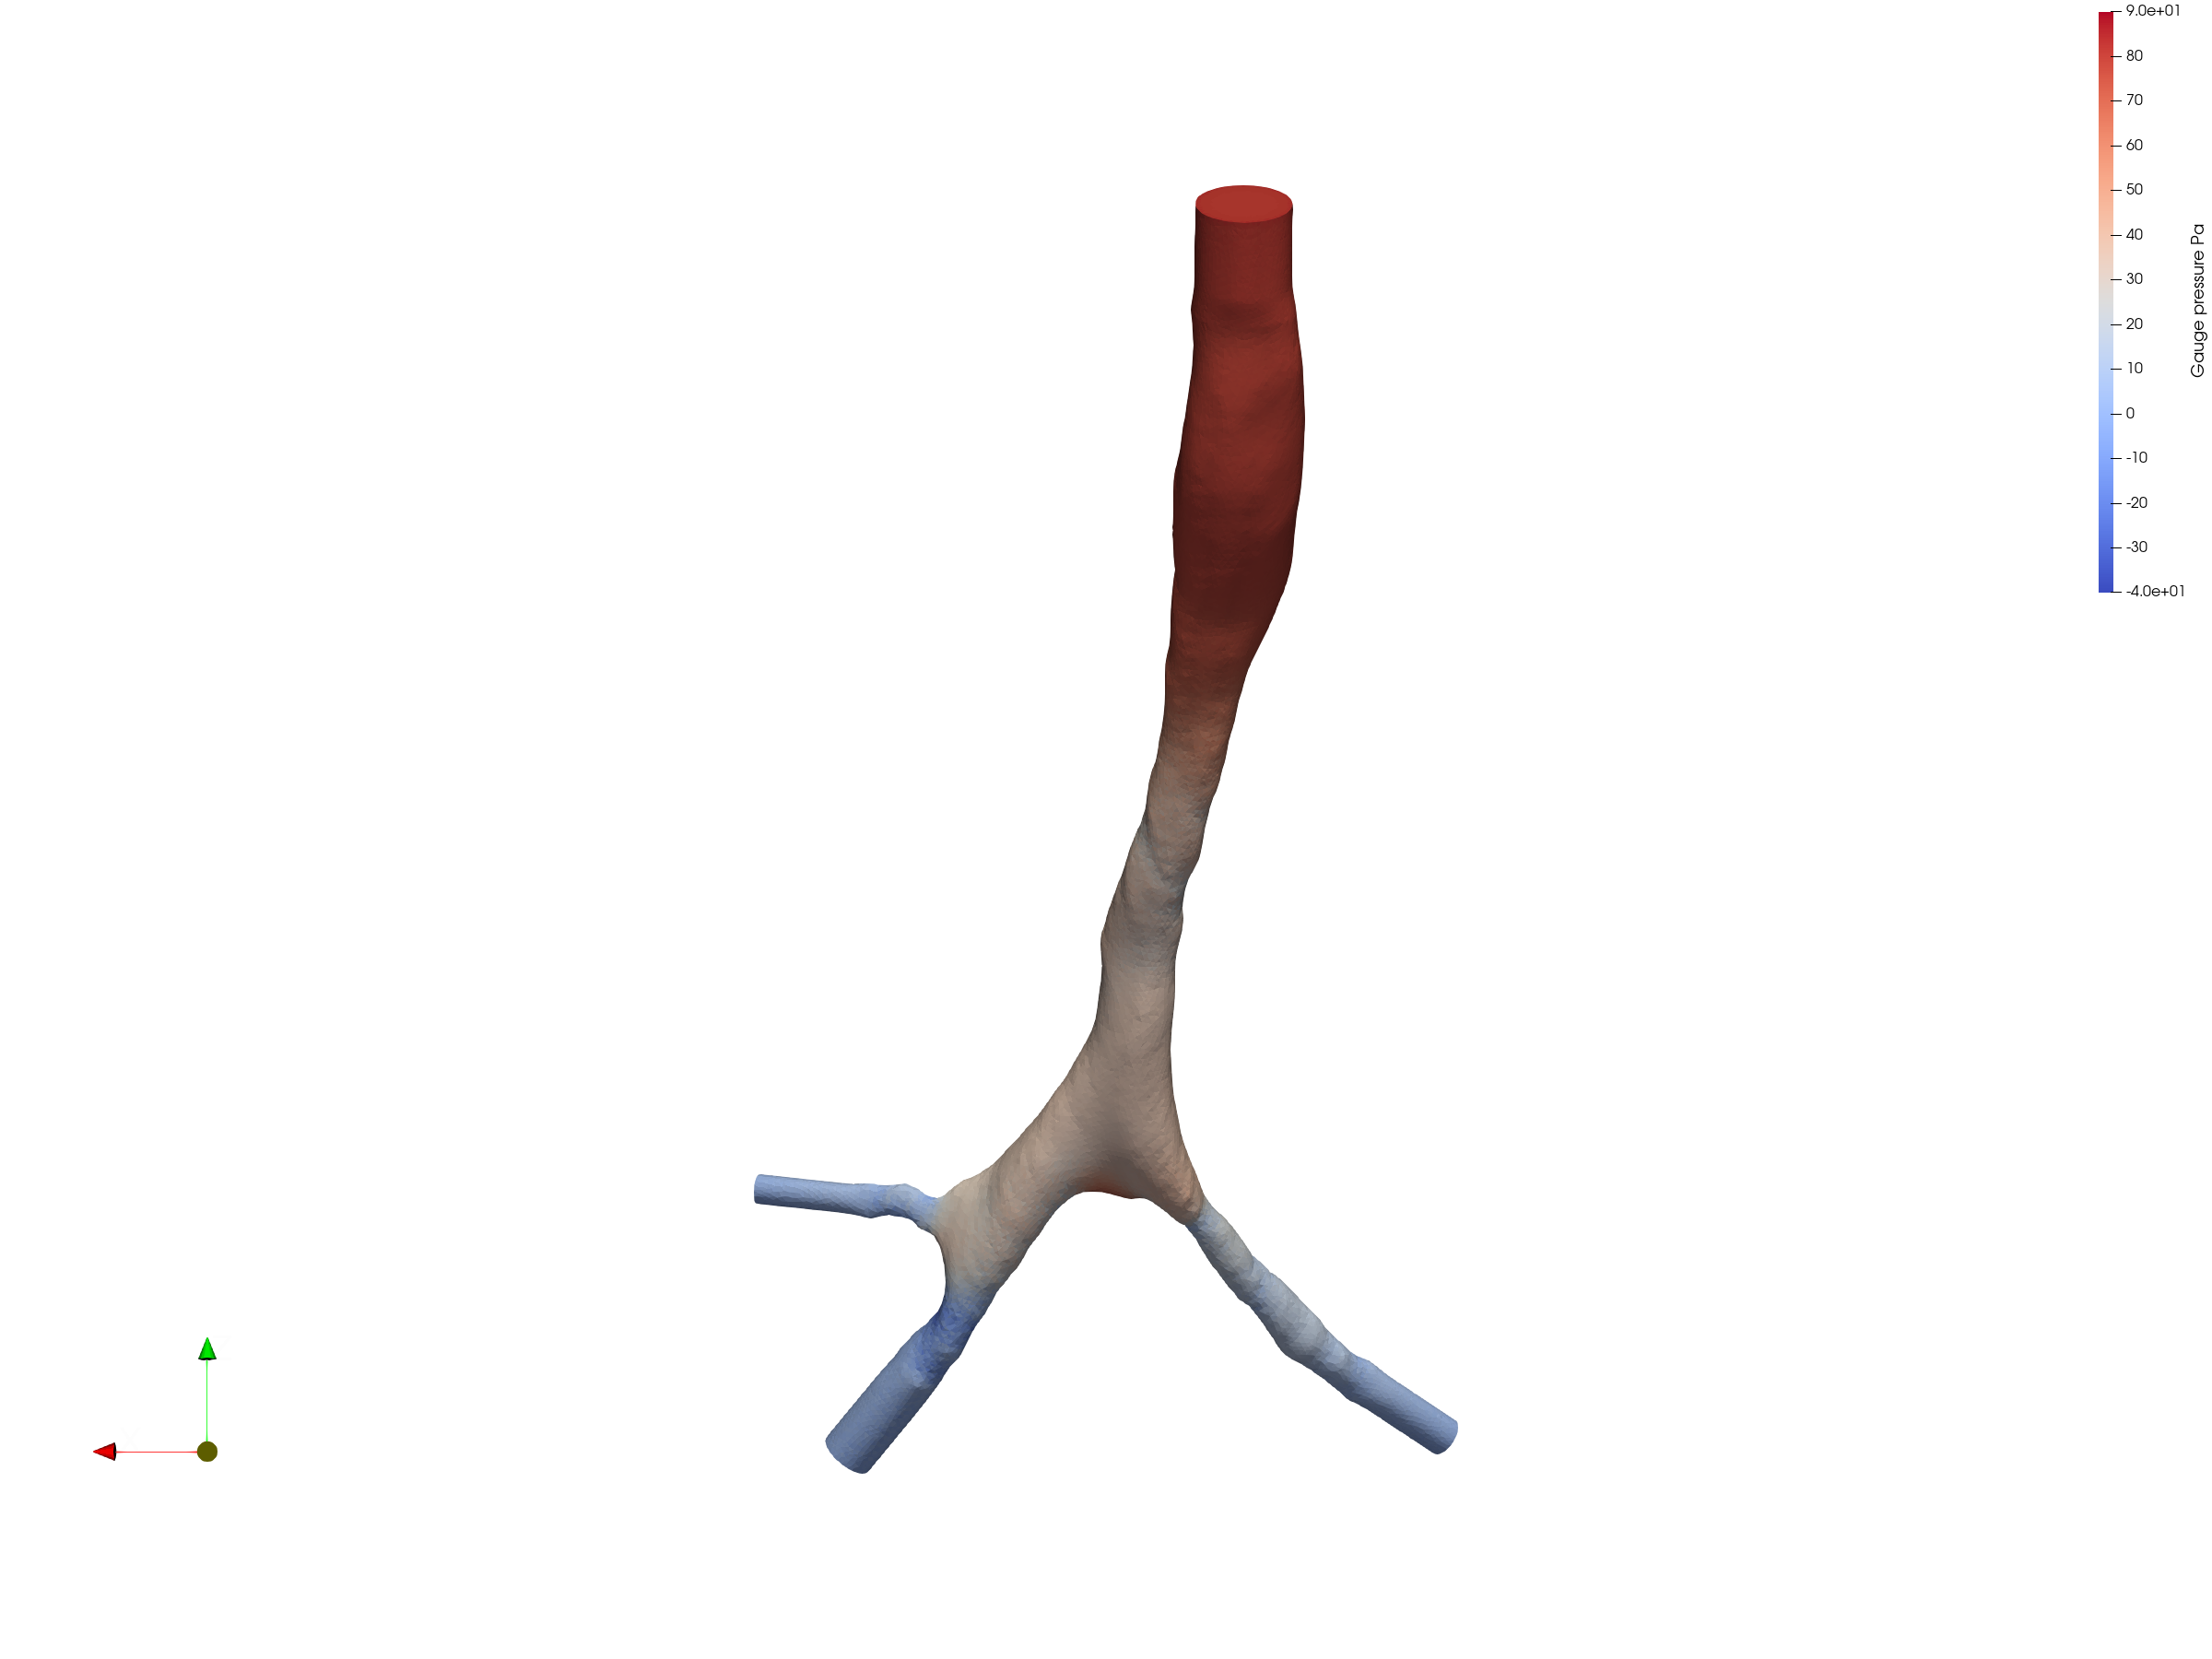
\includegraphics[width=\linewidth,height=0.60\textheight,keepaspectratio]{assignment4_pressure_distribution.png}
  \end{columns}
  \vspace{0.2em}
  \centering\small At \SI{2}{\litre\per\minute}: $\Delta P=\SI{30.95}{\pascal}$, local resistance $=\SI{15.41}{\pascal\per\litre\per\minute}$, peak velocity $=\SI{9.25}{\metre\per\second}$.
\end{frame}

\begin{frame}{Flow distribution emerges from geometry}
  \begin{columns}[T,onlytextwidth]
    \column{0.48\textwidth}
      \begin{block}{Computed distribution}
        \centering\Huge
        $Q_R=73.17\%$\\[0.4em]
        $Q_L=26.83\%$
      \end{block}
    \column{0.48\textwidth}
      \begin{itemize}
        \item Total inlet flow was prescribed.
        \item Every distal outlet had the same zero gauge pressure.
        \item No outlet split was imposed:
          \[
            Q_i\sim\frac{\Delta P}{R_i}.
          \]
        \item Diameter, length, curvature, branch angle, and separation determine effective resistance.
      \end{itemize}
  \end{columns}
  \begin{alertblock}{Interpretation limit}
    This is geometry-driven flow division in the truncated domain, not measured physiological ventilation; peripheral resistance and compliance are absent.
  \end{alertblock}
\end{frame}

\begin{frame}{Transient postoperative proof of concept}
  \begin{columns}[T,onlytextwidth]
    \column{0.62\textwidth}
      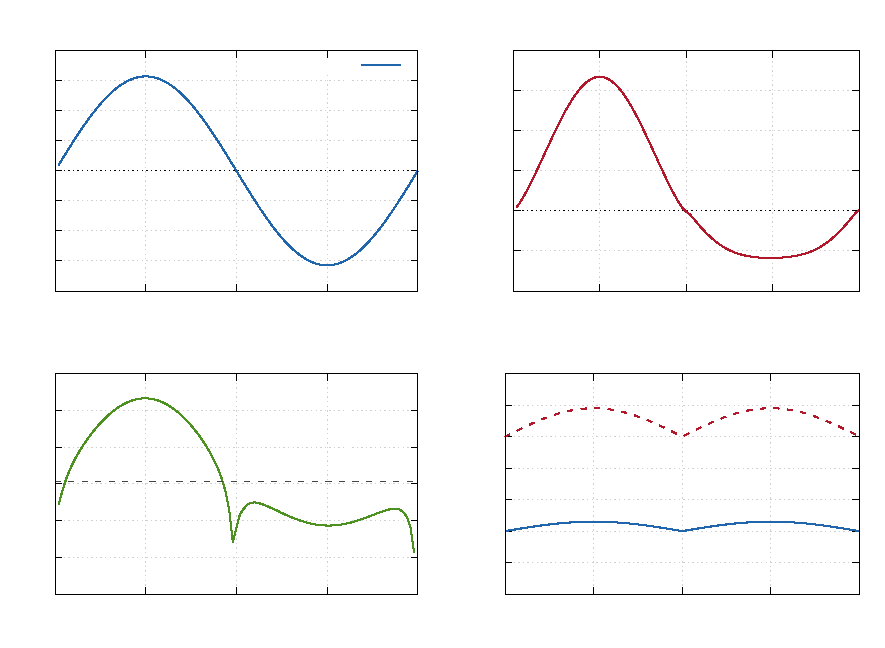
\includegraphics[width=\linewidth,height=0.73\textheight,keepaspectratio]{assignment6_cycle_response.pdf}
    \column{0.35\textwidth}
      \begin{itemize}
        \item Complete \SI{2}{\second} cycle
        \item Peak flow: $\pm\SI{6.29}{\litre\per\minute}$
        \item $\Delta P$: $-58.7$ to \SI{167.4}{\pascal}
        \item $R$: 5.71--26.63 Pa/(L/min)
        \item Near-zero-flow resistance masked
        \item 99.826\% of timesteps met the PIMPLE criterion
      \end{itemize}
  \end{columns}
  \vspace{-0.4em}
  \centering\scriptsize Coarse 0.25 mm PoC, bounded upwind and $\mathrm{Co}_{\max}=5$: qualitative phase trends, not a timestep-independent prediction.
\end{frame}

\begin{frame}{Flow reverses over the breathing cycle}
  \begin{columns}[T,onlytextwidth]
    \column{0.32\textwidth}
      \centering\textbf{Accelerating inspiration}\par
      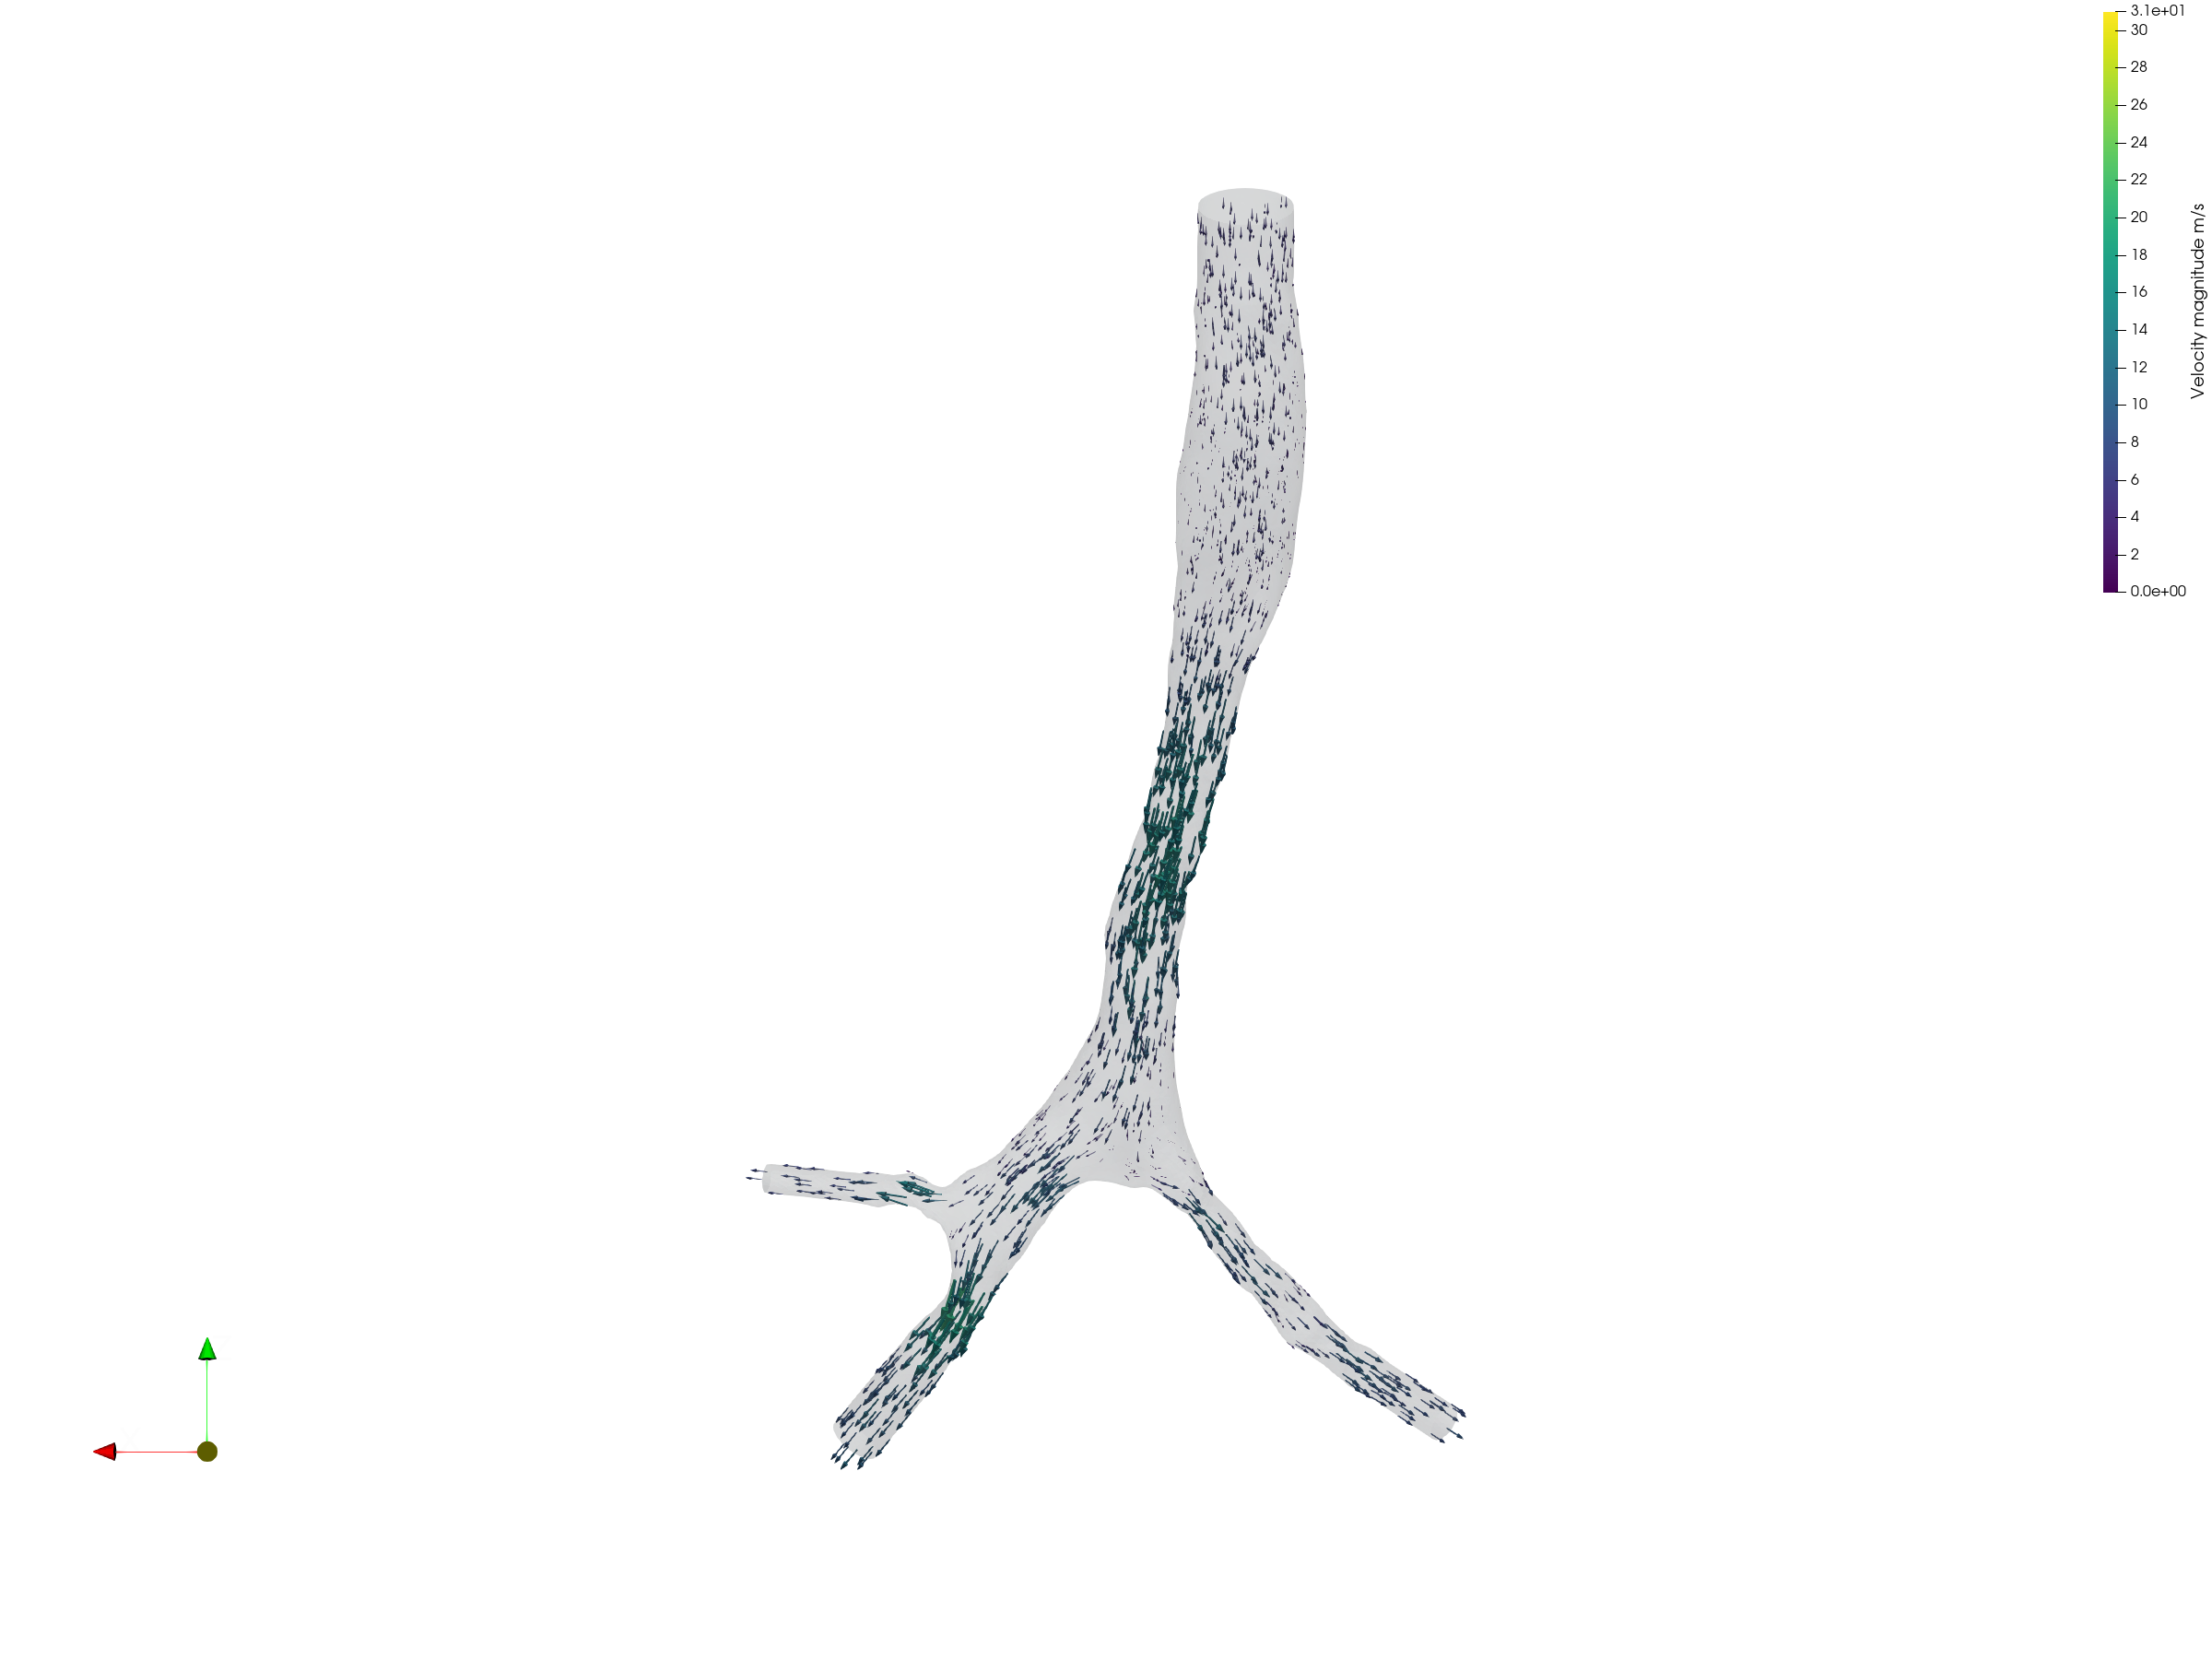
\includegraphics[width=\linewidth,height=0.66\textheight,keepaspectratio]{assignment6_vectors_024.png}
      \small $t=\SI{0.24}{\second}$
    \column{0.32\textwidth}
      \centering\textbf{Peak inspiration}\par
      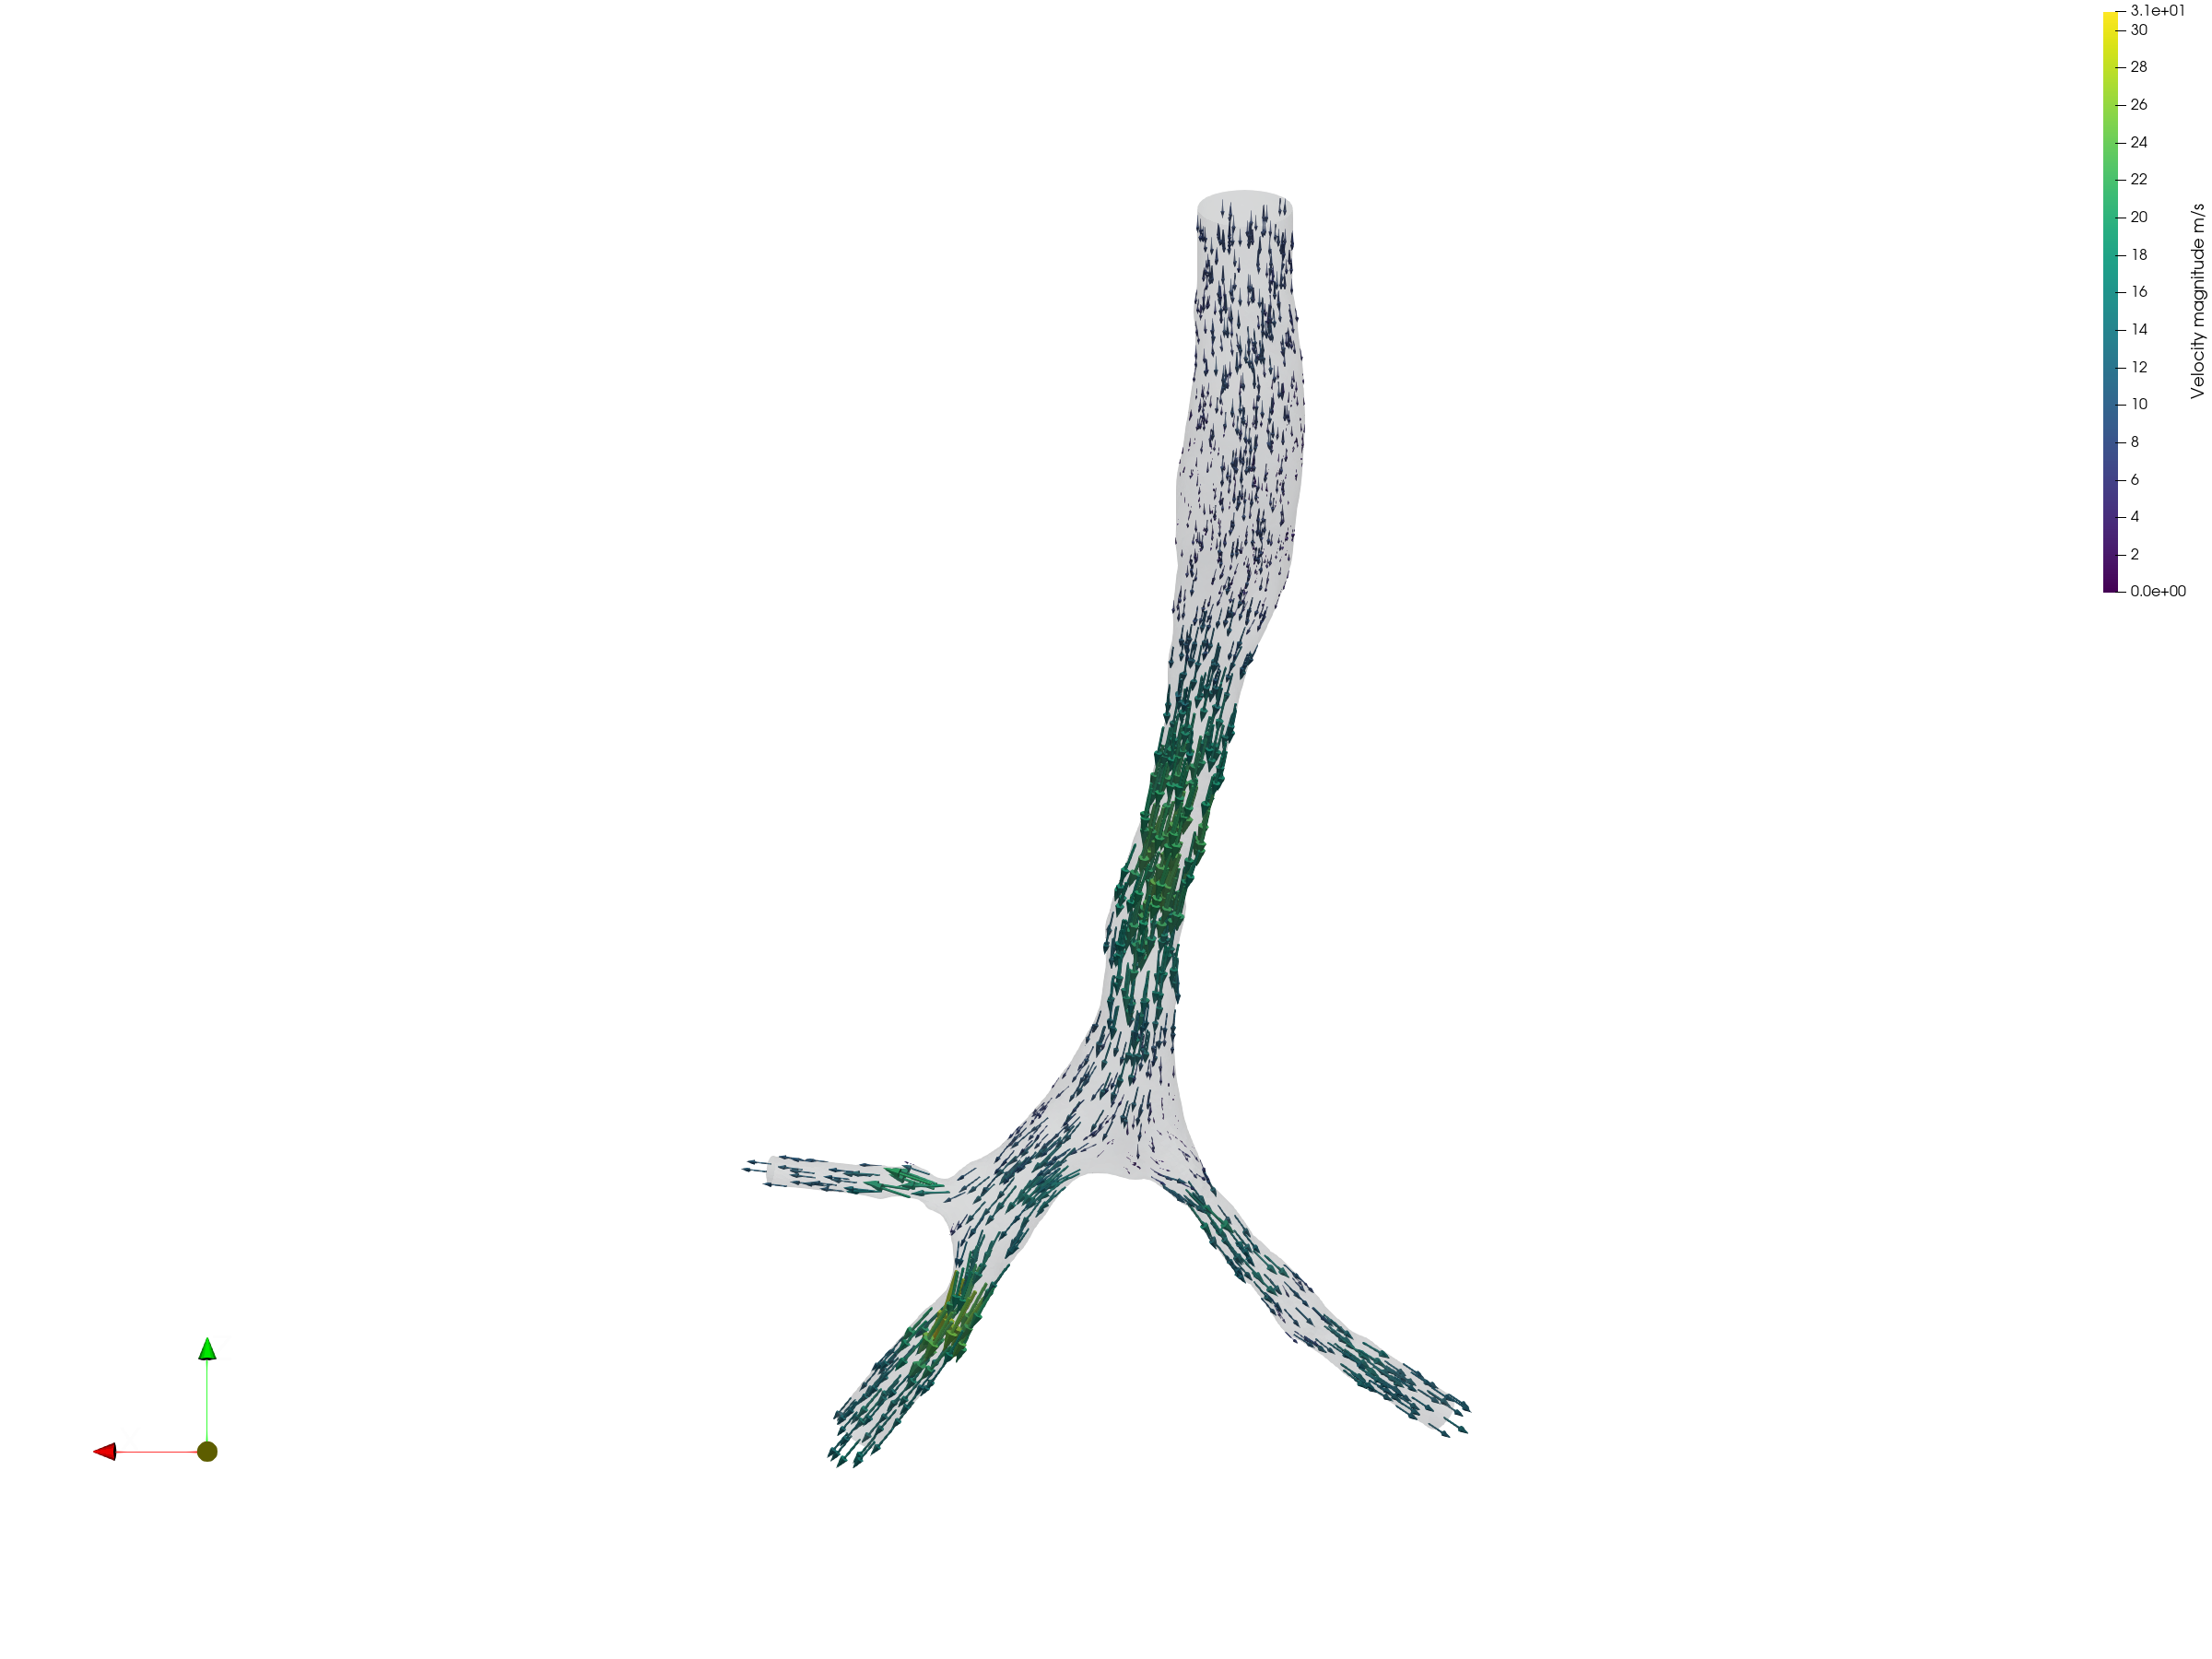
\includegraphics[width=\linewidth,height=0.66\textheight,keepaspectratio]{assignment6_vectors_050.png}
      \small $t=\SI{0.50}{\second}$
    \column{0.32\textwidth}
      \centering\textbf{Peak expiration}\par
      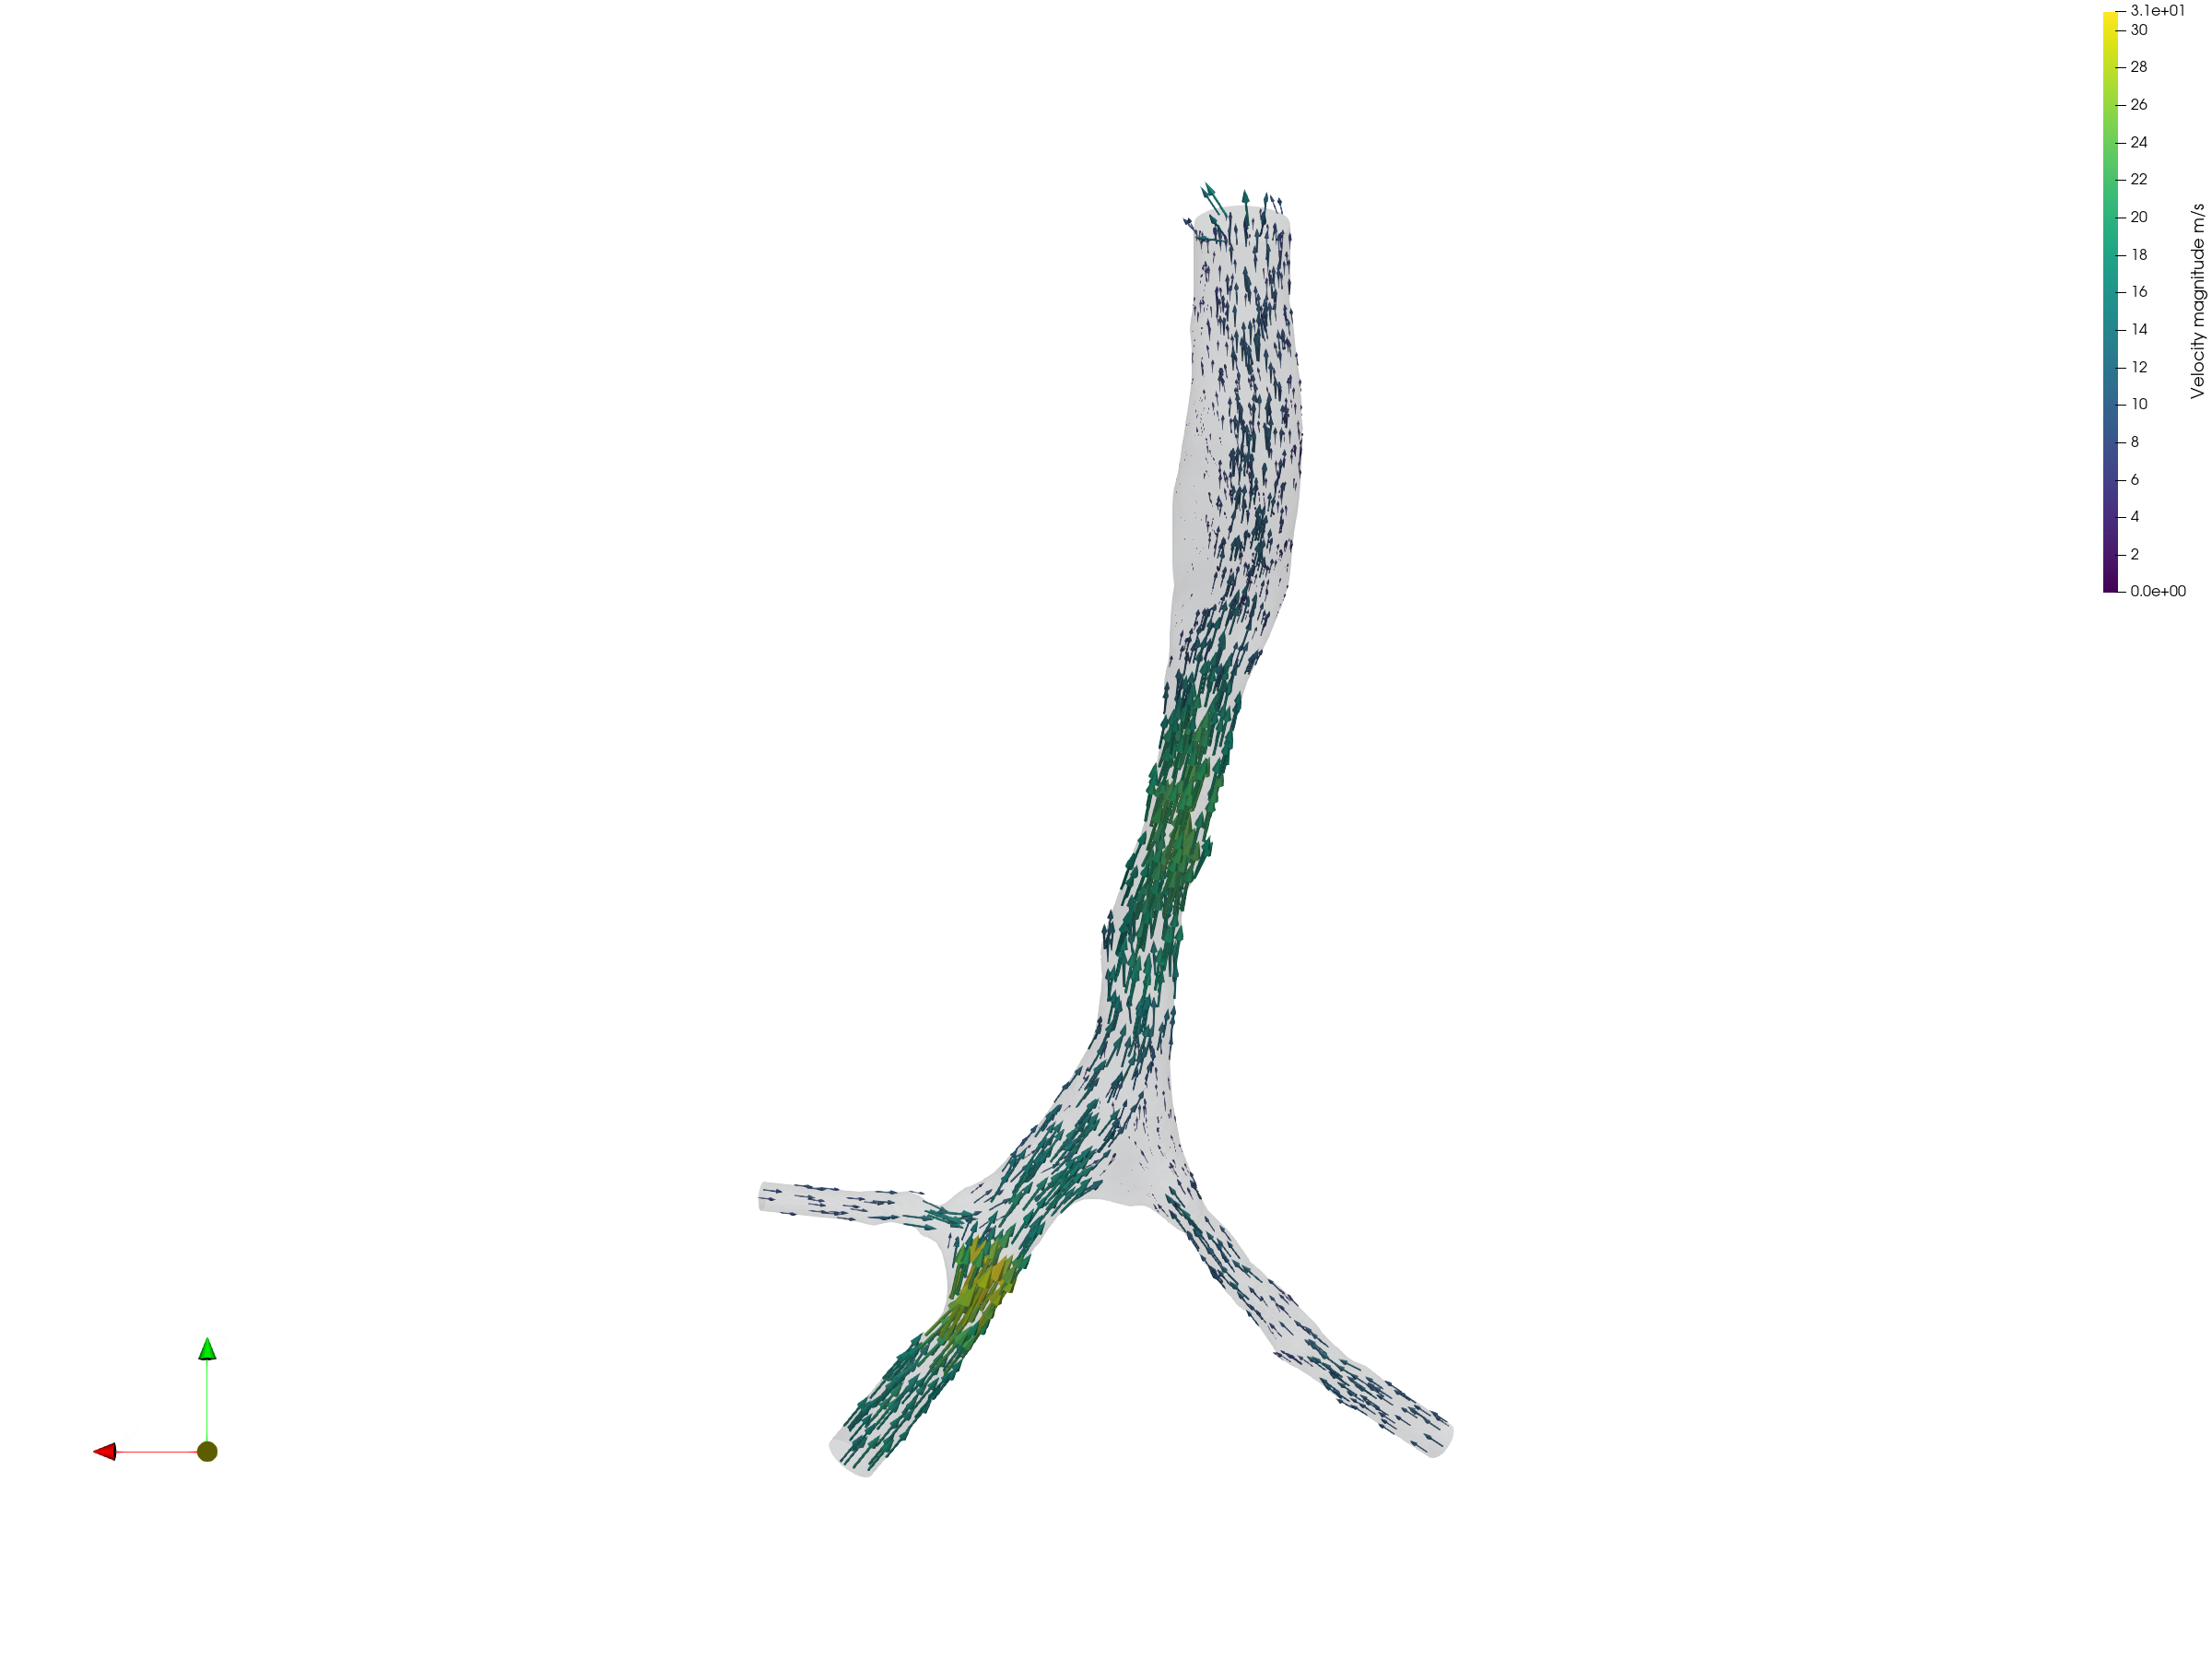
\includegraphics[width=\linewidth,height=0.66\textheight,keepaspectratio]{assignment6_vectors_150.png}
      \small $t=\SI{1.50}{\second}$
  \end{columns}
  \centering\scriptsize Common \SIrange{0}{31}{\metre\per\second} colour scale and vector scale.
\end{frame}

\begin{frame}{Conclusions and limitations}
  \begin{columns}[T,onlytextwidth]
    \column{0.52\textwidth}
      \textbf{Principal findings}
      \begin{itemize}
        \item Surgery increased matched area from 1.813 to \SI{5.169}{\milli\metre\squared}.
        \item The postoperative model produced a marked geometry-driven 73/27 right/left split.
        \item The 0.15 mm mesh balanced sensitivity and computational cost for steady CFD.
        \item The transient workflow resolves the imposed breathing phases as a PoC.
      \end{itemize}
    \column{0.44\textwidth}
      \textbf{Main limitations}
      \begin{itemize}
        \item Static, rigid CT geometry
        \item No peripheral lung impedance
        \item Laminar model
        \item No prism boundary layers
        \item One patient and one initial cycle
        \item Coarse transient fallback at high Courant number
      \end{itemize}
  \end{columns}
  \vfill
  \centering\Large Questions?
\end{frame}

\end{document}
